\documentclass[a4paper]{book}
\usepackage{a4wide}
\usepackage{makeidx}
\usepackage{graphicx}
\usepackage{multicol}
\usepackage{float}
\usepackage{listings}
\usepackage{color}
\usepackage{textcomp}
\usepackage{alltt}
\usepackage{times}
\usepackage[utf8]{inputenc}
\usepackage{doxygen}
\lstset{language=C++,inputencoding=utf8,basicstyle=\footnotesize,breaklines=true,breakatwhitespace=true,tabsize=8,numbers=left }
\makeindex
\setcounter{tocdepth}{3}
\renewcommand{\footrulewidth}{0.4pt}
\begin{document}
\begin{titlepage}
\vspace*{7cm}
\begin{center}
{\Large AstroDeconvolution }\\
\vspace*{1cm}
{\large Generated by Doxygen 1.6.1}\\
\vspace*{0.5cm}
{\small Sun Feb 28 11:39:42 2010}\\
\end{center}
\end{titlepage}
\clearemptydoublepage
\pagenumbering{roman}
\tableofcontents
\clearemptydoublepage
\pagenumbering{arabic}
\chapter{Correction of astro photos by deconvolution}
\label{index}\section{Introduction}\label{index_introduction}
Stars are in principle point sources. However, if we take a picture of stars, we find that the star images have a finite extension. This is caused by the atmosphere and imperfections of the telescope and recording media. This spreading of the star image can be described by {\itshape convolution\/}: \[I(x, y) = \int _{-\infty} ^ {+\infty} \int _{-\infty} ^ {+\infty} PSF(x', y') S(x-x', y-y')dx' dy'\] where $S(x,y)$ is the real star image, $PSF(x,y)$ is the {\itshape Point Spread Function\/} and $I(x,y)$ is the resulting image.

Programs like IRIS allow you to do {\itshape deconvolution\/}, i.e., to reverse the process described above and to get an image that is a better representation of $S(x,y)$. However, this method is restricted to \%PSF that are position independent. Some of the distortions that can occur in image recording have a \%PSF that is position dependent. For instance, coma is a deformation that increases to the edge of the picture. Another example is a picture taken with a telescope mount where the polar axis is not perfectly aligned, causing stars to be recorded as circle segments.

This program is based on the article {\tt Deconvolution with a spatially-\/variant PSF}.\section{The theory}\label{index_theory}
A standard way of doing deconvolution is the {\itshape Lucy-\/Richardson Deconvolution Algorithm\/}. This algorithm starts with an original estimate of the star image $P(x,y)$. This image is then convoluted with the known PSF and the result is compared with the actual image $I(x,y)$. Based on the difference a new estimate of the star image is generated and these steps are repeated until the two images compare well.

By far the fastest way to do the convolutions is by means of the Fast Foerier Transform (FFT). However, this only works the PSF is constant over the area of the image.

As described in {\tt Deconvolution with a spatially-\/variant PSF} it is possible to generate a set of orthogonal base PSF, analogous to generating a set of orthogonal base vectors in an N-\/dimensional vector space, in such a way that each PSF can be expressed as a lineair combination of these base PSF. If we write the base PSF, that are independent of the position in the image as $P_i(x,y$, then we can write \[ P(u, v,x,y) = \sum _ {i = 1} ^ N a_i(u, v, x,y) P_i(x,y) \] where $u$ and $v$ are the coordinates in the image and $x$ and $y$ are trhe coordinates in the PSF.

With this expression we can write the convolution of the star image with the spatially variant PSF as \[ I (x,y) = \sum _{i = 1} ^ N \int _{-\infty} ^ {+\infty} \int _{-\infty} ^ {+\infty} S(u, v) a_i (u, v) p_i (x -u, y - v)du dv \]

Each of the terms in this formula is now a convolution with a PSF that is spatially invariant and and can therefore be calculated with FFT.

This program handles correction of (astro) photos by deconvolution with a spatially-\/variant PSF.\section{The Algorithm}\label{index_algorithm}
The first step is to determine the \%PSF as function of the position in the image. This program does not use theoretical formluas ot parameterized functions for the \%PSF. In stead it assumes that the pixels around a star in the recorded image {\itshape is\/} the PSF. This is done in class PSF. 
\chapter{Namespace Index}
\section{Package List}
Here are the packages with brief descriptions (if available):\begin{DoxyCompactList}
\item\contentsline{section}{{\bf AstroCorrection} }{\pageref{namespace_astro_correction}}{}
\item\contentsline{section}{{\bf AstroCorrection.Properties} }{\pageref{namespace_astro_correction_1_1_properties}}{}
\end{DoxyCompactList}

\chapter{Class Index}
\section{Class Hierarchy}
This inheritance list is sorted roughly, but not completely, alphabetically:\begin{DoxyCompactList}
\item \contentsline{section}{AstroCorrection.CovarianceBuilder}{\pageref{class_astro_correction_1_1_covariance_builder}}{}
\item \contentsline{section}{AstroCorrection.HotellingTransform}{\pageref{class_astro_correction_1_1_hotelling_transform}}{}
\item \contentsline{section}{AstroCorrection.IConvolutable}{\pageref{interface_astro_correction_1_1_i_convolutable}}{}
\begin{DoxyCompactList}
\item \contentsline{section}{AstroCorrection.CompoundPSF}{\pageref{class_astro_correction_1_1_compound_p_s_f}}{}
\item \contentsline{section}{AstroCorrection.PSF}{\pageref{class_astro_correction_1_1_p_s_f}}{}
\end{DoxyCompactList}
\item \contentsline{section}{AstroCorrection.ImageF}{\pageref{class_astro_correction_1_1_image_f}}{}
\item \contentsline{section}{AstroCorrection.ImageScan}{\pageref{class_astro_correction_1_1_image_scan}}{}
\item \contentsline{section}{AstroCorrection.KLCoefficients}{\pageref{class_astro_correction_1_1_k_l_coefficients}}{}
\item \contentsline{section}{AstroCorrection.MainForm}{\pageref{class_astro_correction_1_1_main_form}}{}
\item \contentsline{section}{AstroCorrection.PhotographData}{\pageref{class_astro_correction_1_1_photograph_data}}{}
\item \contentsline{section}{AstroCorrection.PhotographData.PixelData}{\pageref{struct_astro_correction_1_1_photograph_data_1_1_pixel_data}}{}
\item \contentsline{section}{AstroCorrection.PsfWrapper}{\pageref{class_astro_correction_1_1_psf_wrapper}}{}
\item \contentsline{section}{AstroCorrection.Properties.Resources}{\pageref{class_astro_correction_1_1_properties_1_1_resources}}{}
\item \contentsline{section}{AstroCorrection.RichardsonLucyDeconvolution}{\pageref{class_astro_correction_1_1_richardson_lucy_deconvolution}}{}
\item \contentsline{section}{AstroCorrection.RunningAverage}{\pageref{class_astro_correction_1_1_running_average}}{}
\item \contentsline{section}{AstroCorrection.RunningCovariance}{\pageref{class_astro_correction_1_1_running_covariance}}{}
\item \contentsline{section}{AstroCorrection.RunningStatistics}{\pageref{class_astro_correction_1_1_running_statistics}}{}
\item \contentsline{section}{AstroCorrection.ScanLineAnalyzer}{\pageref{class_astro_correction_1_1_scan_line_analyzer}}{}
\item \contentsline{section}{AstroCorrection.SelectablePictureBox}{\pageref{class_astro_correction_1_1_selectable_picture_box}}{}
\item \contentsline{section}{AstroCorrection.Properties.Settings}{\pageref{class_astro_correction_1_1_properties_1_1_settings}}{}
\item \contentsline{section}{AstroCorrection.ShiftingArray$<$ T $>$}{\pageref{class_astro_correction_1_1_shifting_array_3_01_t_01_4}}{}
\end{DoxyCompactList}

\chapter{Class Index}
\section{Class List}
Here are the classes, structs, unions and interfaces with brief descriptions:\begin{DoxyCompactList}
\item\contentsline{section}{{\bf AstroCorrection.CompoundPSF} (Spatially Variant \doxyref{PSF}{p.}{class_astro_correction_1_1_p_s_f}, with Karhunen-\/Loève decomposition )}{\pageref{class_astro_correction_1_1_compound_p_s_f}}{}
\item\contentsline{section}{{\bf AstroCorrection.CovarianceBuilder} }{\pageref{class_astro_correction_1_1_covariance_builder}}{}
\item\contentsline{section}{{\bf AstroCorrection.HotellingTransform} }{\pageref{class_astro_correction_1_1_hotelling_transform}}{}
\item\contentsline{section}{{\bf AstroCorrection.IConvolutable} (Interface that allows Convolution into an \doxyref{ImageF}{p.}{class_astro_correction_1_1_image_f} )}{\pageref{interface_astro_correction_1_1_i_convolutable}}{}
\item\contentsline{section}{{\bf AstroCorrection.ImageF} (Monochrome image where the pixels are stored as floating point numbers )}{\pageref{class_astro_correction_1_1_image_f}}{}
\item\contentsline{section}{{\bf AstroCorrection.ImageScan} (Show \doxyref{PSF}{p.}{class_astro_correction_1_1_p_s_f} images in a 'film strip' )}{\pageref{class_astro_correction_1_1_image_scan}}{}
\item\contentsline{section}{{\bf AstroCorrection.KLCoefficients} (Base class for Coefficients in Karhunen-\/Loève PSF decomposition )}{\pageref{class_astro_correction_1_1_k_l_coefficients}}{}
\item\contentsline{section}{{\bf AstroCorrection.MainForm} }{\pageref{class_astro_correction_1_1_main_form}}{}
\item\contentsline{section}{{\bf AstroCorrection.PhotographData} (Wrapper around photograph data )}{\pageref{class_astro_correction_1_1_photograph_data}}{}
\item\contentsline{section}{{\bf AstroCorrection.PhotographData.PixelData} (Data about a single pixel )}{\pageref{struct_astro_correction_1_1_photograph_data_1_1_pixel_data}}{}
\item\contentsline{section}{{\bf AstroCorrection.PSF} (PixelData Spread Function )}{\pageref{class_astro_correction_1_1_p_s_f}}{}
\item\contentsline{section}{{\bf AstroCorrection.PsfWrapper} }{\pageref{class_astro_correction_1_1_psf_wrapper}}{}
\item\contentsline{section}{{\bf AstroCorrection.Properties.Resources} (A strongly-\/typed resource class, for looking up localized strings, etc )}{\pageref{class_astro_correction_1_1_properties_1_1_resources}}{}
\item\contentsline{section}{{\bf AstroCorrection.RichardsonLucyDeconvolution} }{\pageref{class_astro_correction_1_1_richardson_lucy_deconvolution}}{}
\item\contentsline{section}{{\bf AstroCorrection.RunningAverage} }{\pageref{class_astro_correction_1_1_running_average}}{}
\item\contentsline{section}{{\bf AstroCorrection.RunningCovariance} }{\pageref{class_astro_correction_1_1_running_covariance}}{}
\item\contentsline{section}{{\bf AstroCorrection.RunningStatistics} }{\pageref{class_astro_correction_1_1_running_statistics}}{}
\item\contentsline{section}{{\bf AstroCorrection.ScanLineAnalyzer} (Analyze a small piece of an image along a scan line (horizontal) )}{\pageref{class_astro_correction_1_1_scan_line_analyzer}}{}
\item\contentsline{section}{{\bf AstroCorrection.SelectablePictureBox} }{\pageref{class_astro_correction_1_1_selectable_picture_box}}{}
\item\contentsline{section}{{\bf AstroCorrection.Properties.Settings} }{\pageref{class_astro_correction_1_1_properties_1_1_settings}}{}
\item\contentsline{section}{{\bf AstroCorrection.ShiftingArray$<$ T $>$} }{\pageref{class_astro_correction_1_1_shifting_array_3_01_t_01_4}}{}
\end{DoxyCompactList}

\chapter{File Index}
\section{File List}
Here is a list of all files with brief descriptions:\begin{DoxyCompactList}
\item\contentsline{section}{C:/Users/Joost/Documents/Development/MyProjects/AstroCorrection/AstroCorrection/{\bf CompoundPSF.cs} }{\pageref{_compound_p_s_f_8cs}}{}
\item\contentsline{section}{C:/Users/Joost/Documents/Development/MyProjects/AstroCorrection/AstroCorrection/{\bf CovarianceBuilder.cs} }{\pageref{_covariance_builder_8cs}}{}
\item\contentsline{section}{C:/Users/Joost/Documents/Development/MyProjects/AstroCorrection/AstroCorrection/{\bf HotellingTransform.cs} }{\pageref{_hotelling_transform_8cs}}{}
\item\contentsline{section}{C:/Users/Joost/Documents/Development/MyProjects/AstroCorrection/AstroCorrection/{\bf IConvolutable.cs} }{\pageref{_i_convolutable_8cs}}{}
\item\contentsline{section}{C:/Users/Joost/Documents/Development/MyProjects/AstroCorrection/AstroCorrection/{\bf ImageF.cs} }{\pageref{_image_f_8cs}}{}
\item\contentsline{section}{C:/Users/Joost/Documents/Development/MyProjects/AstroCorrection/AstroCorrection/{\bf ImageScan.cs} }{\pageref{_image_scan_8cs}}{}
\item\contentsline{section}{C:/Users/Joost/Documents/Development/MyProjects/AstroCorrection/AstroCorrection/{\bf KLCoefficients.cs} }{\pageref{_k_l_coefficients_8cs}}{}
\item\contentsline{section}{C:/Users/Joost/Documents/Development/MyProjects/AstroCorrection/AstroCorrection/{\bf MainForm.cs} }{\pageref{_main_form_8cs}}{}
\item\contentsline{section}{C:/Users/Joost/Documents/Development/MyProjects/AstroCorrection/AstroCorrection/{\bf MainForm.Designer.cs} }{\pageref{_main_form_8_designer_8cs}}{}
\item\contentsline{section}{C:/Users/Joost/Documents/Development/MyProjects/AstroCorrection/AstroCorrection/{\bf PhotographData.cs} }{\pageref{_photograph_data_8cs}}{}
\item\contentsline{section}{C:/Users/Joost/Documents/Development/MyProjects/AstroCorrection/AstroCorrection/{\bf Program.cs} }{\pageref{_program_8cs}}{}
\item\contentsline{section}{C:/Users/Joost/Documents/Development/MyProjects/AstroCorrection/AstroCorrection/{\bf PSF.cs} }{\pageref{_p_s_f_8cs}}{}
\item\contentsline{section}{C:/Users/Joost/Documents/Development/MyProjects/AstroCorrection/AstroCorrection/{\bf PsfWrapper.cs} }{\pageref{_psf_wrapper_8cs}}{}
\item\contentsline{section}{C:/Users/Joost/Documents/Development/MyProjects/AstroCorrection/AstroCorrection/{\bf RichardsonLucyDeconvolution.cs} }{\pageref{_richardson_lucy_deconvolution_8cs}}{}
\item\contentsline{section}{C:/Users/Joost/Documents/Development/MyProjects/AstroCorrection/AstroCorrection/{\bf RunningAverage.cs} }{\pageref{_running_average_8cs}}{}
\item\contentsline{section}{C:/Users/Joost/Documents/Development/MyProjects/AstroCorrection/AstroCorrection/{\bf RunningCovariance.cs} }{\pageref{_running_covariance_8cs}}{}
\item\contentsline{section}{C:/Users/Joost/Documents/Development/MyProjects/AstroCorrection/AstroCorrection/{\bf RunningVariance.cs} }{\pageref{_running_variance_8cs}}{}
\item\contentsline{section}{C:/Users/Joost/Documents/Development/MyProjects/AstroCorrection/AstroCorrection/{\bf ScanLineAnalyzer.cs} }{\pageref{_scan_line_analyzer_8cs}}{}
\item\contentsline{section}{C:/Users/Joost/Documents/Development/MyProjects/AstroCorrection/AstroCorrection/{\bf SelectablePictureBox.cs} }{\pageref{_selectable_picture_box_8cs}}{}
\item\contentsline{section}{C:/Users/Joost/Documents/Development/MyProjects/AstroCorrection/AstroCorrection/{\bf ShiftingArray.cs} }{\pageref{_shifting_array_8cs}}{}
\item\contentsline{section}{C:/Users/Joost/Documents/Development/MyProjects/AstroCorrection/AstroCorrection/Properties/{\bf AssemblyInfo.cs} }{\pageref{_assembly_info_8cs}}{}
\item\contentsline{section}{C:/Users/Joost/Documents/Development/MyProjects/AstroCorrection/AstroCorrection/Properties/{\bf Resources.Designer.cs} }{\pageref{_resources_8_designer_8cs}}{}
\item\contentsline{section}{C:/Users/Joost/Documents/Development/MyProjects/AstroCorrection/AstroCorrection/Properties/{\bf Settings.Designer.cs} }{\pageref{_settings_8_designer_8cs}}{}
\end{DoxyCompactList}

\chapter{Namespace Documentation}
\section{Package AstroCorrection}
\label{namespace_astro_correction}\index{AstroCorrection@{AstroCorrection}}
\subsection*{Packages}
\begin{DoxyCompactItemize}
\item 
package {\bf Properties}
\end{DoxyCompactItemize}
\subsection*{Classes}
\begin{DoxyCompactItemize}
\item 
class {\bf CompoundPSF}
\begin{DoxyCompactList}\small\item\em Spatially Variant \doxyref{PSF}{p.}{class_astro_correction_1_1_p_s_f}, with Karhunen-\/Loève decomposition. \item\end{DoxyCompactList}\item 
class {\bf CovarianceBuilder}
\item 
class {\bf HotellingTransform}
\item 
interface {\bf IConvolutable}
\begin{DoxyCompactList}\small\item\em Interface that allows Convolution into an \doxyref{ImageF}{p.}{class_astro_correction_1_1_image_f}. \item\end{DoxyCompactList}\item 
class {\bf ImageF}
\begin{DoxyCompactList}\small\item\em Monochrome image where the pixels are stored as floating point numbers. \item\end{DoxyCompactList}\item 
class {\bf ImageScan}
\begin{DoxyCompactList}\small\item\em Show \doxyref{PSF}{p.}{class_astro_correction_1_1_p_s_f} images in a 'film strip'. \item\end{DoxyCompactList}\item 
class {\bf KLCoefficients}
\begin{DoxyCompactList}\small\item\em Base class for Coefficients in Karhunen-\/Loève PSF decomposition. \item\end{DoxyCompactList}\item 
class {\bf MainForm}
\item 
class {\bf PhotographData}
\begin{DoxyCompactList}\small\item\em Wrapper around photograph data. \item\end{DoxyCompactList}\item 
class {\bfseries Program}
\item 
class {\bf PSF}
\begin{DoxyCompactList}\small\item\em PixelData Spread Function. \item\end{DoxyCompactList}\item 
class {\bf PsfWrapper}
\item 
class {\bf RichardsonLucyDeconvolution}
\item 
class {\bf RunningAverage}
\item 
class {\bf RunningCovariance}
\item 
class {\bf RunningStatistics}
\item 
class {\bf ScanLineAnalyzer}
\begin{DoxyCompactList}\small\item\em Analyze a small piece of an image along a scan line (horizontal). \item\end{DoxyCompactList}\item 
class {\bf SelectablePictureBox}
\item 
class {\bf ShiftingArray$<$ T $>$}
\end{DoxyCompactItemize}

\section{Package AstroCorrection.Properties}
\label{namespace_astro_correction_1_1_properties}\index{AstroCorrection.Properties@{AstroCorrection.Properties}}
\subsection*{Classes}
\begin{DoxyCompactItemize}
\item 
class {\bf Resources}
\begin{DoxyCompactList}\small\item\em A strongly-\/typed resource class, for looking up localized strings, etc. \item\end{DoxyCompactList}\item 
class {\bf Settings}
\end{DoxyCompactItemize}

\chapter{Class Documentation}
\section{AstroCorrection.CompoundPSF Class Reference}
\label{class_astro_correction_1_1_compound_p_s_f}\index{AstroCorrection::CompoundPSF@{AstroCorrection::CompoundPSF}}


Spatially Variant \doxyref{PSF}{p.}{class_astro_correction_1_1_p_s_f}, with Karhunen-\/Loève decomposition.  
Inheritance diagram for AstroCorrection.CompoundPSF::\begin{figure}[H]
\begin{center}
\leavevmode
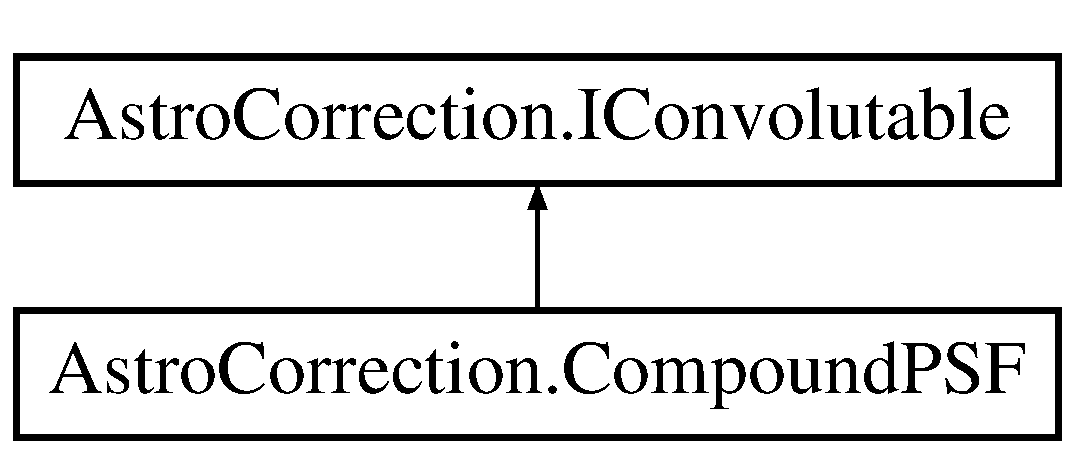
\includegraphics[height=2cm]{class_astro_correction_1_1_compound_p_s_f}
\end{center}
\end{figure}
\subsection*{Public Member Functions}
\begin{DoxyCompactItemize}
\item 
{\bf CompoundPSF} ()
\begin{DoxyCompactList}\small\item\em Constructor. \item\end{DoxyCompactList}\item 
void {\bf Construct} (List$<$ {\bf PSF} $>$ psf, {\bf KLCoefficients} aPrototype)
\begin{DoxyCompactList}\small\item\em Construct from a list of \doxyref{PSF}{p.}{class_astro_correction_1_1_p_s_f}. \item\end{DoxyCompactList}\item 
{\bf ImageF} {\bf Convolute} ({\bf ImageF} image)
\begin{DoxyCompactList}\small\item\em Convolute the object with the \doxyref{ImageF}{p.}{class_astro_correction_1_1_image_f}. \item\end{DoxyCompactList}\end{DoxyCompactItemize}


\subsection{Detailed Description}
Spatially Variant \doxyref{PSF}{p.}{class_astro_correction_1_1_p_s_f}, with Karhunen-\/Loève decomposition. 

Definition at line 12 of file CompoundPSF.cs.

\subsection{Constructor \& Destructor Documentation}
\index{AstroCorrection::CompoundPSF@{AstroCorrection::CompoundPSF}!CompoundPSF@{CompoundPSF}}
\index{CompoundPSF@{CompoundPSF}!AstroCorrection::CompoundPSF@{AstroCorrection::CompoundPSF}}
\subsubsection[{CompoundPSF}]{\setlength{\rightskip}{0pt plus 5cm}AstroCorrection.CompoundPSF.CompoundPSF ()}\label{class_astro_correction_1_1_compound_p_s_f_a3a0201ec80dbc336282681df0015daef}


Constructor. 

Definition at line 18 of file CompoundPSF.cs.

\subsection{Member Function Documentation}
\index{AstroCorrection::CompoundPSF@{AstroCorrection::CompoundPSF}!Construct@{Construct}}
\index{Construct@{Construct}!AstroCorrection::CompoundPSF@{AstroCorrection::CompoundPSF}}
\subsubsection[{Construct}]{\setlength{\rightskip}{0pt plus 5cm}void AstroCorrection.CompoundPSF.Construct (List$<$ {\bf PSF} $>$ {\em psf}, \/  {\bf KLCoefficients} {\em aPrototype})}\label{class_astro_correction_1_1_compound_p_s_f_a163da36b0461523ecfa01a335e9d3b68}


Construct from a list of \doxyref{PSF}{p.}{class_astro_correction_1_1_p_s_f}. 
\begin{DoxyParams}{Parameters}
\item[{\em psf}]The list to contruct the \doxyref{CompoundPSF}{p.}{class_astro_correction_1_1_compound_p_s_f} from \item[{\em aPrototype}]Prototype of the coefficients to use in decomposition \end{DoxyParams}


Definition at line 30 of file CompoundPSF.cs.\index{AstroCorrection::CompoundPSF@{AstroCorrection::CompoundPSF}!Convolute@{Convolute}}
\index{Convolute@{Convolute}!AstroCorrection::CompoundPSF@{AstroCorrection::CompoundPSF}}
\subsubsection[{Convolute}]{\setlength{\rightskip}{0pt plus 5cm}{\bf ImageF} AstroCorrection.CompoundPSF.Convolute ({\bf ImageF} {\em image})}\label{class_astro_correction_1_1_compound_p_s_f_afff7554ee0a0d7ce659b87fd236ddff4}


Convolute the object with the \doxyref{ImageF}{p.}{class_astro_correction_1_1_image_f}. 
\begin{DoxyParams}{Parameters}
\item[{\em image}]The image to convolute with\end{DoxyParams}
\begin{DoxyReturn}{Returns}
The result of the convlution 
\end{DoxyReturn}


Implements {\bf AstroCorrection.IConvolutable} \doxyref{}{p.}{interface_astro_correction_1_1_i_convolutable_a01a503ab4927505350bc1865d4b8dd35}.

Definition at line 36 of file CompoundPSF.cs.

The documentation for this class was generated from the following file:\begin{DoxyCompactItemize}
\item 
C:/Users/Joost/Documents/Development/MyProjects/AstroCorrection/AstroCorrection/{\bf CompoundPSF.cs}\end{DoxyCompactItemize}

\section{AstroCorrection.CovarianceBuilder Class Reference}
\label{class_astro_correction_1_1_covariance_builder}\index{AstroCorrection::CovarianceBuilder@{AstroCorrection::CovarianceBuilder}}
\subsection*{Public Member Functions}
\begin{DoxyCompactItemize}
\item 
{\bf CovarianceBuilder} ({\bf PhotographData} data)
\item 
Matrix {\bf Create} ()
\end{DoxyCompactItemize}


\subsection{Detailed Description}


Definition at line 13 of file CovarianceBuilder.cs.

\subsection{Constructor \& Destructor Documentation}
\index{AstroCorrection::CovarianceBuilder@{AstroCorrection::CovarianceBuilder}!CovarianceBuilder@{CovarianceBuilder}}
\index{CovarianceBuilder@{CovarianceBuilder}!AstroCorrection::CovarianceBuilder@{AstroCorrection::CovarianceBuilder}}
\subsubsection[{CovarianceBuilder}]{\setlength{\rightskip}{0pt plus 5cm}AstroCorrection.CovarianceBuilder.CovarianceBuilder ({\bf PhotographData} {\em data})}\label{class_astro_correction_1_1_covariance_builder_a9fcc5d6904a014be52c960a1823a9457}


Definition at line 22 of file CovarianceBuilder.cs.

\subsection{Member Function Documentation}
\index{AstroCorrection::CovarianceBuilder@{AstroCorrection::CovarianceBuilder}!Create@{Create}}
\index{Create@{Create}!AstroCorrection::CovarianceBuilder@{AstroCorrection::CovarianceBuilder}}
\subsubsection[{Create}]{\setlength{\rightskip}{0pt plus 5cm}Matrix AstroCorrection.CovarianceBuilder.Create ()}\label{class_astro_correction_1_1_covariance_builder_aceeea96620c3efb0be54ac5cfd50b5c9}


Definition at line 37 of file CovarianceBuilder.cs.

The documentation for this class was generated from the following file:\begin{DoxyCompactItemize}
\item 
C:/Users/Joost/Documents/Development/MyProjects/AstroCorrection/AstroCorrection/{\bf CovarianceBuilder.cs}\end{DoxyCompactItemize}

\section{AstroCorrection.HotellingTransform Class Reference}
\label{class_astro_correction_1_1_hotelling_transform}\index{AstroCorrection::HotellingTransform@{AstroCorrection::HotellingTransform}}
\subsection*{Classes}
\begin{DoxyCompactItemize}
\item 
struct {\bfseries EigenElement}
\end{DoxyCompactItemize}
\subsection*{Public Member Functions}
\begin{DoxyCompactItemize}
\item 
double {\bf Mean} (int idx)
\item 
{\bf HotellingTransform} (int size)
\item 
{\bf HotellingTransform} (IEnumerable$<$ double[$\,$]$>$ vectors)
\item 
void {\bf Add} (double[$\,$] X)
\item 
double[$\,$] {\bf Transform} (double[$\,$] X)
\end{DoxyCompactItemize}
\subsection*{Properties}
\begin{DoxyCompactItemize}
\item 
int {\bf Size}\hspace{0.3cm}{\ttfamily  [get, set]}
\end{DoxyCompactItemize}


\subsection{Detailed Description}


Definition at line 11 of file HotellingTransform.cs.

\subsection{Constructor \& Destructor Documentation}
\index{AstroCorrection::HotellingTransform@{AstroCorrection::HotellingTransform}!HotellingTransform@{HotellingTransform}}
\index{HotellingTransform@{HotellingTransform}!AstroCorrection::HotellingTransform@{AstroCorrection::HotellingTransform}}
\subsubsection[{HotellingTransform}]{\setlength{\rightskip}{0pt plus 5cm}AstroCorrection.HotellingTransform.HotellingTransform (int {\em size})}\label{class_astro_correction_1_1_hotelling_transform_abc13063ff1f6b757524d4f18de7b50a2}


Definition at line 36 of file HotellingTransform.cs.\index{AstroCorrection::HotellingTransform@{AstroCorrection::HotellingTransform}!HotellingTransform@{HotellingTransform}}
\index{HotellingTransform@{HotellingTransform}!AstroCorrection::HotellingTransform@{AstroCorrection::HotellingTransform}}
\subsubsection[{HotellingTransform}]{\setlength{\rightskip}{0pt plus 5cm}AstroCorrection.HotellingTransform.HotellingTransform (IEnumerable$<$ double[$\,$]$>$ {\em vectors})}\label{class_astro_correction_1_1_hotelling_transform_ac3a759dac4bbd72897aea286520f3b41}


Definition at line 41 of file HotellingTransform.cs.

\subsection{Member Function Documentation}
\index{AstroCorrection::HotellingTransform@{AstroCorrection::HotellingTransform}!Add@{Add}}
\index{Add@{Add}!AstroCorrection::HotellingTransform@{AstroCorrection::HotellingTransform}}
\subsubsection[{Add}]{\setlength{\rightskip}{0pt plus 5cm}void AstroCorrection.HotellingTransform.Add (double[$\,$] {\em X})}\label{class_astro_correction_1_1_hotelling_transform_ad78364d0eac5bd4429f02db95aef7ebe}


Definition at line 67 of file HotellingTransform.cs.\index{AstroCorrection::HotellingTransform@{AstroCorrection::HotellingTransform}!Mean@{Mean}}
\index{Mean@{Mean}!AstroCorrection::HotellingTransform@{AstroCorrection::HotellingTransform}}
\subsubsection[{Mean}]{\setlength{\rightskip}{0pt plus 5cm}double AstroCorrection.HotellingTransform.Mean (int {\em idx})}\label{class_astro_correction_1_1_hotelling_transform_a0dc476137dec9835b7b2c9e33b5bf012}


Definition at line 30 of file HotellingTransform.cs.\index{AstroCorrection::HotellingTransform@{AstroCorrection::HotellingTransform}!Transform@{Transform}}
\index{Transform@{Transform}!AstroCorrection::HotellingTransform@{AstroCorrection::HotellingTransform}}
\subsubsection[{Transform}]{\setlength{\rightskip}{0pt plus 5cm}double [$\,$] AstroCorrection.HotellingTransform.Transform (double[$\,$] {\em X})}\label{class_astro_correction_1_1_hotelling_transform_a7eb74ec91bb8f2f6c6800df7d00daad0}


Definition at line 133 of file HotellingTransform.cs.

\subsection{Property Documentation}
\index{AstroCorrection::HotellingTransform@{AstroCorrection::HotellingTransform}!Size@{Size}}
\index{Size@{Size}!AstroCorrection::HotellingTransform@{AstroCorrection::HotellingTransform}}
\subsubsection[{Size}]{\setlength{\rightskip}{0pt plus 5cm}int AstroCorrection.HotellingTransform.Size\hspace{0.3cm}{\ttfamily  [get, set]}}\label{class_astro_correction_1_1_hotelling_transform_a30f3433fd432028404f894b19de7dc57}


Definition at line 19 of file HotellingTransform.cs.

The documentation for this class was generated from the following file:\begin{DoxyCompactItemize}
\item 
C:/Users/Joost/Documents/Development/MyProjects/AstroCorrection/AstroCorrection/{\bf HotellingTransform.cs}\end{DoxyCompactItemize}

\section{AstroCorrection.IConvolutable Interface Reference}
\label{interface_astro_correction_1_1_i_convolutable}\index{AstroCorrection::IConvolutable@{AstroCorrection::IConvolutable}}


Interface that allows Convolution into an \doxyref{ImageF}{p.}{class_astro_correction_1_1_image_f}.  
Inheritance diagram for AstroCorrection.IConvolutable::\begin{figure}[H]
\begin{center}
\leavevmode
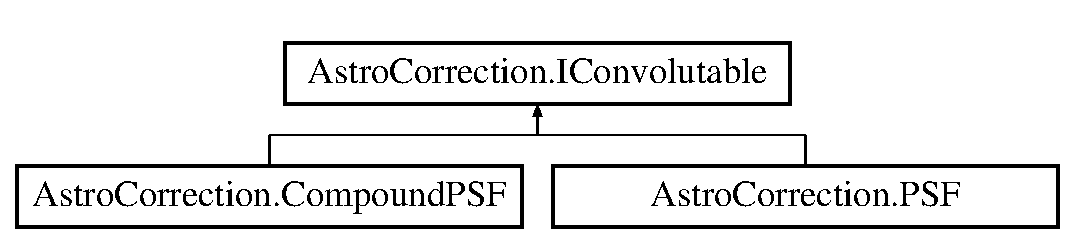
\includegraphics[height=2cm]{interface_astro_correction_1_1_i_convolutable}
\end{center}
\end{figure}
\subsection*{Public Member Functions}
\begin{DoxyCompactItemize}
\item 
{\bf ImageF} {\bf Convolute} ({\bf ImageF} image)
\begin{DoxyCompactList}\small\item\em Convolute the object with the \doxyref{ImageF}{p.}{class_astro_correction_1_1_image_f}. \item\end{DoxyCompactList}\end{DoxyCompactItemize}


\subsection{Detailed Description}
Interface that allows Convolution into an \doxyref{ImageF}{p.}{class_astro_correction_1_1_image_f}. 

Definition at line 12 of file IConvolutable.cs.

\subsection{Member Function Documentation}
\index{AstroCorrection::IConvolutable@{AstroCorrection::IConvolutable}!Convolute@{Convolute}}
\index{Convolute@{Convolute}!AstroCorrection::IConvolutable@{AstroCorrection::IConvolutable}}
\subsubsection[{Convolute}]{\setlength{\rightskip}{0pt plus 5cm}{\bf ImageF} AstroCorrection.IConvolutable.Convolute ({\bf ImageF} {\em image})}\label{interface_astro_correction_1_1_i_convolutable_a01a503ab4927505350bc1865d4b8dd35}


Convolute the object with the \doxyref{ImageF}{p.}{class_astro_correction_1_1_image_f}. 
\begin{DoxyParams}{Parameters}
\item[{\em image}]The image to convolute with\end{DoxyParams}
\begin{DoxyReturn}{Returns}
The result of the convlution 
\end{DoxyReturn}


Implemented in {\bf AstroCorrection.CompoundPSF} \doxyref{}{p.}{class_astro_correction_1_1_compound_p_s_f_afff7554ee0a0d7ce659b87fd236ddff4}, and {\bf AstroCorrection.PSF} \doxyref{}{p.}{class_astro_correction_1_1_p_s_f_a81fbd1fefd705253807d8edc6502fed0}.

The documentation for this interface was generated from the following file:\begin{DoxyCompactItemize}
\item 
C:/Users/Joost/Documents/Development/MyProjects/AstroCorrection/AstroCorrection/{\bf IConvolutable.cs}\end{DoxyCompactItemize}

\section{AstroCorrection.ImageF Class Reference}
\label{class_astro_correction_1_1_image_f}\index{AstroCorrection::ImageF@{AstroCorrection::ImageF}}


Monochrome image where the pixels are stored as floating point numbers.  
\subsection*{Public Member Functions}
\begin{DoxyCompactItemize}
\item 
{\bf ImageF} {\bf Add} ({\bf ImageF} rhs)
\begin{DoxyCompactList}\small\item\em Add an \doxyref{ImageF}{p.}{class_astro_correction_1_1_image_f} pixelwise to this object. \item\end{DoxyCompactList}\item 
{\bf ImageF} {\bf Convolute} ({\bf PSF} psf)
\begin{DoxyCompactList}\small\item\em Convolute the PSF into this \doxyref{ImageF}{p.}{class_astro_correction_1_1_image_f}. \item\end{DoxyCompactList}\end{DoxyCompactItemize}
\subsection*{Static Public Member Functions}
\begin{DoxyCompactItemize}
\item 
static {\bf ImageF} {\bf FromArray} (double[,] array)
\begin{DoxyCompactList}\small\item\em Create an \doxyref{ImageF}{p.}{class_astro_correction_1_1_image_f} from a two-\/dimensional array. \item\end{DoxyCompactList}\item 
static unsafe {\bf ImageF} {\bf FromBitmap} (Bitmap bm)
\begin{DoxyCompactList}\small\item\em Creat an \doxyref{ImageF}{p.}{class_astro_correction_1_1_image_f} from a Bitmap. \item\end{DoxyCompactList}\item 
static {\bf ImageF} {\bf operator+} ({\bf ImageF} lhs, {\bf ImageF} rhs)
\begin{DoxyCompactList}\small\item\em Add two \doxyref{ImageF}{p.}{class_astro_correction_1_1_image_f} objects pixel by pixel. \item\end{DoxyCompactList}\end{DoxyCompactItemize}
\subsection*{Properties}
\begin{DoxyCompactItemize}
\item 
double {\bf this} [int x, int y]\hspace{0.3cm}{\ttfamily  [get]}
\begin{DoxyCompactList}\small\item\em Get the value of a pixel. \item\end{DoxyCompactList}\item 
int {\bf Width}\hspace{0.3cm}{\ttfamily  [get]}
\begin{DoxyCompactList}\small\item\em Get the width of the image. \item\end{DoxyCompactList}\item 
int {\bf Height}\hspace{0.3cm}{\ttfamily  [get]}
\begin{DoxyCompactList}\small\item\em Get the height of the image. \item\end{DoxyCompactList}\end{DoxyCompactItemize}


\subsection{Detailed Description}
Monochrome image where the pixels are stored as floating point numbers. The image is read-\/only and can only be created by static methods or (protected) constructors 

Definition at line 17 of file ImageF.cs.

\subsection{Member Function Documentation}
\index{AstroCorrection::ImageF@{AstroCorrection::ImageF}!Add@{Add}}
\index{Add@{Add}!AstroCorrection::ImageF@{AstroCorrection::ImageF}}
\subsubsection[{Add}]{\setlength{\rightskip}{0pt plus 5cm}{\bf ImageF} AstroCorrection.ImageF.Add ({\bf ImageF} {\em rhs})}\label{class_astro_correction_1_1_image_f_aed9906052fa592697fc1cd7351c44a4a}


Add an \doxyref{ImageF}{p.}{class_astro_correction_1_1_image_f} pixelwise to this object. 
\begin{DoxyParams}{Parameters}
\item[{\em rhs}]\doxyref{ImageF}{p.}{class_astro_correction_1_1_image_f} object to add\end{DoxyParams}
\begin{DoxyReturn}{Returns}
The result of the addition 
\end{DoxyReturn}


Definition at line 147 of file ImageF.cs.\index{AstroCorrection::ImageF@{AstroCorrection::ImageF}!Convolute@{Convolute}}
\index{Convolute@{Convolute}!AstroCorrection::ImageF@{AstroCorrection::ImageF}}
\subsubsection[{Convolute}]{\setlength{\rightskip}{0pt plus 5cm}{\bf ImageF} AstroCorrection.ImageF.Convolute ({\bf PSF} {\em psf})}\label{class_astro_correction_1_1_image_f_a5a9fa9933194b4807e40ef677f6dc0e9}


Convolute the PSF into this \doxyref{ImageF}{p.}{class_astro_correction_1_1_image_f}. 
\begin{DoxyParams}{Parameters}
\item[{\em psf}]The PSF to convolve\end{DoxyParams}
\begin{DoxyReturn}{Returns}
The result of the convolution 
\end{DoxyReturn}


Definition at line 184 of file ImageF.cs.\index{AstroCorrection::ImageF@{AstroCorrection::ImageF}!FromArray@{FromArray}}
\index{FromArray@{FromArray}!AstroCorrection::ImageF@{AstroCorrection::ImageF}}
\subsubsection[{FromArray}]{\setlength{\rightskip}{0pt plus 5cm}static {\bf ImageF} AstroCorrection.ImageF.FromArray (double {\em array}[,])\hspace{0.3cm}{\ttfamily  [static]}}\label{class_astro_correction_1_1_image_f_a4e739e3415fdfeb1d39d57bc32f68f63}


Create an \doxyref{ImageF}{p.}{class_astro_correction_1_1_image_f} from a two-\/dimensional array. 
\begin{DoxyParams}{Parameters}
\item[{\em array}]The two dimensional arry to wrap in an \doxyref{ImageF}{p.}{class_astro_correction_1_1_image_f} \end{DoxyParams}
\begin{DoxyReturn}{Returns}
The created \doxyref{ImageF}{p.}{class_astro_correction_1_1_image_f} 
\end{DoxyReturn}


Definition at line 92 of file ImageF.cs.\index{AstroCorrection::ImageF@{AstroCorrection::ImageF}!FromBitmap@{FromBitmap}}
\index{FromBitmap@{FromBitmap}!AstroCorrection::ImageF@{AstroCorrection::ImageF}}
\subsubsection[{FromBitmap}]{\setlength{\rightskip}{0pt plus 5cm}static unsafe {\bf ImageF} AstroCorrection.ImageF.FromBitmap (Bitmap {\em bm})\hspace{0.3cm}{\ttfamily  [static]}}\label{class_astro_correction_1_1_image_f_a270534ff1a59e954a15418226c5a627a}


Creat an \doxyref{ImageF}{p.}{class_astro_correction_1_1_image_f} from a Bitmap. The function takes the intensity of each pixel by adding the RGB values


\begin{DoxyParams}{Parameters}
\item[{\em bm}]The bitmap to wrap \end{DoxyParams}
\begin{DoxyReturn}{Returns}
The created \doxyref{ImageF}{p.}{class_astro_correction_1_1_image_f}
\end{DoxyReturn}
\begin{DoxyNote}{Note}
The funcion is declared {\itshape unsafe\/} since it uses pointers to the bitmap data to speed-\/up the process ofg conversion 
\end{DoxyNote}


Definition at line 111 of file ImageF.cs.\index{AstroCorrection::ImageF@{AstroCorrection::ImageF}!operator+@{operator+}}
\index{operator+@{operator+}!AstroCorrection::ImageF@{AstroCorrection::ImageF}}
\subsubsection[{operator+}]{\setlength{\rightskip}{0pt plus 5cm}static {\bf ImageF} AstroCorrection.ImageF.operator+ ({\bf ImageF} {\em lhs}, \/  {\bf ImageF} {\em rhs})\hspace{0.3cm}{\ttfamily  [static]}}\label{class_astro_correction_1_1_image_f_a770ed7cf86d352c53452b0002321f358}


Add two \doxyref{ImageF}{p.}{class_astro_correction_1_1_image_f} objects pixel by pixel. 
\begin{DoxyParams}{Parameters}
\item[{\em lhs}]First of the \doxyref{ImageF}{p.}{class_astro_correction_1_1_image_f} objects \item[{\em rhs}]Second of the \doxyref{ImageF}{p.}{class_astro_correction_1_1_image_f} objects\end{DoxyParams}
\begin{DoxyReturn}{Returns}
The result of the addition 
\end{DoxyReturn}


Definition at line 171 of file ImageF.cs.

\subsection{Property Documentation}
\index{AstroCorrection::ImageF@{AstroCorrection::ImageF}!Height@{Height}}
\index{Height@{Height}!AstroCorrection::ImageF@{AstroCorrection::ImageF}}
\subsubsection[{Height}]{\setlength{\rightskip}{0pt plus 5cm}int AstroCorrection.ImageF.Height\hspace{0.3cm}{\ttfamily  [get]}}\label{class_astro_correction_1_1_image_f_ae30acbd6946f49875b4763ae02545c27}


Get the height of the image. 

Definition at line 56 of file ImageF.cs.\index{AstroCorrection::ImageF@{AstroCorrection::ImageF}!this@{this}}
\index{this@{this}!AstroCorrection::ImageF@{AstroCorrection::ImageF}}
\subsubsection[{this}]{\setlength{\rightskip}{0pt plus 5cm}double AstroCorrection.ImageF.this[int x, int y]\hspace{0.3cm}{\ttfamily  [get]}}\label{class_astro_correction_1_1_image_f_adfe147a34cac7d6c6134267bb71d8053}


Get the value of a pixel. 
\begin{DoxyParams}{Parameters}
\item[{\em x}]X-\/value of the pixel \item[{\em y}]Y-\/value of the pixel\end{DoxyParams}
\begin{DoxyReturn}{Returns}
the value of the pixel at \{x,y\} 
\end{DoxyReturn}


Definition at line 32 of file ImageF.cs.\index{AstroCorrection::ImageF@{AstroCorrection::ImageF}!Width@{Width}}
\index{Width@{Width}!AstroCorrection::ImageF@{AstroCorrection::ImageF}}
\subsubsection[{Width}]{\setlength{\rightskip}{0pt plus 5cm}int AstroCorrection.ImageF.Width\hspace{0.3cm}{\ttfamily  [get]}}\label{class_astro_correction_1_1_image_f_a1d069d87c92b0608803c93b3f49792cd}


Get the width of the image. 

Definition at line 44 of file ImageF.cs.

The documentation for this class was generated from the following file:\begin{DoxyCompactItemize}
\item 
C:/Users/Joost/Documents/Development/MyProjects/AstroCorrection/AstroCorrection/{\bf ImageF.cs}\end{DoxyCompactItemize}

\section{AstroCorrection.ImageScan Class Reference}
\label{class_astro_correction_1_1_image_scan}\index{AstroCorrection::ImageScan@{AstroCorrection::ImageScan}}


Show \doxyref{PSF}{p.}{class_astro_correction_1_1_p_s_f} images in a 'film strip'.  
\subsection*{Public Member Functions}
\begin{DoxyCompactItemize}
\item 
{\bf ImageScan} ()
\item 
void {\bf Add} ({\bf PsfWrapper} aPsf)
\item 
{\bf PsfWrapper} {\bf GetPsf} (int idx)
\end{DoxyCompactItemize}
\subsection*{Properties}
\begin{DoxyCompactItemize}
\item 
{\bf PsfWrapper} {\bf PSF}\hspace{0.3cm}{\ttfamily  [get, set]}
\end{DoxyCompactItemize}


\subsection{Detailed Description}
Show \doxyref{PSF}{p.}{class_astro_correction_1_1_p_s_f} images in a 'film strip'. 

Definition at line 14 of file ImageScan.cs.

\subsection{Constructor \& Destructor Documentation}
\index{AstroCorrection::ImageScan@{AstroCorrection::ImageScan}!ImageScan@{ImageScan}}
\index{ImageScan@{ImageScan}!AstroCorrection::ImageScan@{AstroCorrection::ImageScan}}
\subsubsection[{ImageScan}]{\setlength{\rightskip}{0pt plus 5cm}AstroCorrection.ImageScan.ImageScan ()}\label{class_astro_correction_1_1_image_scan_a4ebcc2fa159d8fb07ea6ed44fe0166cb}
Constructor 

Definition at line 30 of file ImageScan.cs.

\subsection{Member Function Documentation}
\index{AstroCorrection::ImageScan@{AstroCorrection::ImageScan}!Add@{Add}}
\index{Add@{Add}!AstroCorrection::ImageScan@{AstroCorrection::ImageScan}}
\subsubsection[{Add}]{\setlength{\rightskip}{0pt plus 5cm}void AstroCorrection.ImageScan.Add ({\bf PsfWrapper} {\em aPsf})}\label{class_astro_correction_1_1_image_scan_abbfe687cddc32add7922a7bd68eab83d}
Adda \doxyref{PSF}{p.}{class_astro_correction_1_1_p_s_f} to the images being shown


\begin{DoxyParams}{Parameters}
\item[{\em aPsf}]The \doxyref{PSF}{p.}{class_astro_correction_1_1_p_s_f} to add \end{DoxyParams}


Definition at line 53 of file ImageScan.cs.\index{AstroCorrection::ImageScan@{AstroCorrection::ImageScan}!GetPsf@{GetPsf}}
\index{GetPsf@{GetPsf}!AstroCorrection::ImageScan@{AstroCorrection::ImageScan}}
\subsubsection[{GetPsf}]{\setlength{\rightskip}{0pt plus 5cm}{\bf PsfWrapper} AstroCorrection.ImageScan.GetPsf (int {\em idx})}\label{class_astro_correction_1_1_image_scan_acbc40b8113bef73b625360b3be4f599f}


Definition at line 65 of file ImageScan.cs.

\subsection{Property Documentation}
\index{AstroCorrection::ImageScan@{AstroCorrection::ImageScan}!PSF@{PSF}}
\index{PSF@{PSF}!AstroCorrection::ImageScan@{AstroCorrection::ImageScan}}
\subsubsection[{PSF}]{\setlength{\rightskip}{0pt plus 5cm}{\bf PsfWrapper} AstroCorrection.ImageScan.PSF\hspace{0.3cm}{\ttfamily  [get, set]}}\label{class_astro_correction_1_1_image_scan_a253b723b70e138a570d9b8be4d0f8c33}
Currently selected \doxyref{PSF}{p.}{class_astro_correction_1_1_p_s_f} 

Definition at line 22 of file ImageScan.cs.

The documentation for this class was generated from the following file:\begin{DoxyCompactItemize}
\item 
C:/Users/Joost/Documents/Development/MyProjects/AstroCorrection/AstroCorrection/{\bf ImageScan.cs}\end{DoxyCompactItemize}

\section{AstroCorrection.KLCoefficients Class Reference}
\label{class_astro_correction_1_1_k_l_coefficients}\index{AstroCorrection::KLCoefficients@{AstroCorrection::KLCoefficients}}


Base class for Coefficients in Karhunen-\/Loève PSF decomposition.  
\subsection*{Properties}
\begin{DoxyCompactItemize}
\item 
{\bf ImageF} {\bf Expansion}\hspace{0.3cm}{\ttfamily  [get, set]}
\begin{DoxyCompactList}\small\item\em Get the coefficients expanded to rectangular coordinates. \item\end{DoxyCompactList}\end{DoxyCompactItemize}


\subsection{Detailed Description}
Base class for Coefficients in Karhunen-\/Loève PSF decomposition. These are the coefficients $a_i$ in the expression \[ P(u, v, x, y) = \sum _ {i = 1} ^ N a_i(u, v, x, y) p_i(x,y) \]

The class contains methods to 

Definition at line 19 of file KLCoefficients.cs.

\subsection{Property Documentation}
\index{AstroCorrection::KLCoefficients@{AstroCorrection::KLCoefficients}!Expansion@{Expansion}}
\index{Expansion@{Expansion}!AstroCorrection::KLCoefficients@{AstroCorrection::KLCoefficients}}
\subsubsection[{Expansion}]{\setlength{\rightskip}{0pt plus 5cm}{\bf ImageF} AstroCorrection.KLCoefficients.Expansion\hspace{0.3cm}{\ttfamily  [get, set]}}\label{class_astro_correction_1_1_k_l_coefficients_a1a6d79b74362ab5f842497eef2c66304}


Get the coefficients expanded to rectangular coordinates. Note that setting this property is private. 

Definition at line 28 of file KLCoefficients.cs.

The documentation for this class was generated from the following file:\begin{DoxyCompactItemize}
\item 
C:/Users/Joost/Documents/Development/MyProjects/AstroCorrection/AstroCorrection/{\bf KLCoefficients.cs}\end{DoxyCompactItemize}

\section{AstroCorrection.MainForm Class Reference}
\label{class_astro_correction_1_1_main_form}\index{AstroCorrection::MainForm@{AstroCorrection::MainForm}}
\subsection*{Public Member Functions}
\begin{DoxyCompactItemize}
\item 
{\bf MainForm} ()
\end{DoxyCompactItemize}


\subsection{Detailed Description}


Definition at line 16 of file MainForm.cs.

\subsection{Constructor \& Destructor Documentation}
\index{AstroCorrection::MainForm@{AstroCorrection::MainForm}!MainForm@{MainForm}}
\index{MainForm@{MainForm}!AstroCorrection::MainForm@{AstroCorrection::MainForm}}
\subsubsection[{MainForm}]{\setlength{\rightskip}{0pt plus 5cm}AstroCorrection.MainForm.MainForm ()}\label{class_astro_correction_1_1_main_form_a579713e9d84777dfa0694c4c1286e291}


Definition at line 22 of file MainForm.cs.

The documentation for this class was generated from the following file:\begin{DoxyCompactItemize}
\item 
C:/Users/Joost/Documents/Development/MyProjects/AstroCorrection/AstroCorrection/{\bf MainForm.cs}\end{DoxyCompactItemize}

\section{AstroCorrection.PhotographData Class Reference}
\label{class_astro_correction_1_1_photograph_data}\index{AstroCorrection::PhotographData@{AstroCorrection::PhotographData}}


Wrapper around photograph data.  
\subsection*{Classes}
\begin{DoxyCompactItemize}
\item 
struct {\bf PixelData}
\begin{DoxyCompactList}\small\item\em Data about a single pixel. \item\end{DoxyCompactList}\end{DoxyCompactItemize}
\subsection*{Public Member Functions}
\begin{DoxyCompactItemize}
\item 
{\bf PhotographData} ()
\begin{DoxyCompactList}\small\item\em Default Constructor. \item\end{DoxyCompactList}\item 
{\bf PhotographData} (string aImage)
\begin{DoxyCompactList}\small\item\em Constructor. \item\end{DoxyCompactList}\item 
void {\bf AddPsf} ({\bf PsfWrapper} aPsf)
\begin{DoxyCompactList}\small\item\em Add a \doxyref{PSF}{p.}{class_astro_correction_1_1_p_s_f} to the data. \item\end{DoxyCompactList}\item 
void {\bf Save} (string aFileName)
\begin{DoxyCompactList}\small\item\em Save the data to a file. \item\end{DoxyCompactList}\end{DoxyCompactItemize}
\subsection*{Static Public Member Functions}
\begin{DoxyCompactItemize}
\item 
static {\bf PhotographData} {\bf Load} (string aFileName)
\begin{DoxyCompactList}\small\item\em Load the data from a file. \item\end{DoxyCompactList}\end{DoxyCompactItemize}
\subsection*{Properties}
\begin{DoxyCompactItemize}
\item 
string {\bf Image}\hspace{0.3cm}{\ttfamily  [get, set]}
\begin{DoxyCompactList}\small\item\em Path to the image being analyzed. \item\end{DoxyCompactList}\item 
List$<$ {\bf PsfWrapper} $>$ {\bf PSFs}\hspace{0.3cm}{\ttfamily  [get, set]}
\begin{DoxyCompactList}\small\item\em List of the PSFs in the image. \item\end{DoxyCompactList}\item 
int {\bf NPsf}\hspace{0.3cm}{\ttfamily  [get]}
\begin{DoxyCompactList}\small\item\em Number of \doxyref{PSF}{p.}{class_astro_correction_1_1_p_s_f} associated with the image. \item\end{DoxyCompactList}\item 
IEnumerable$<$ {\bf PixelData} $>$ {\bf AllPixels}\hspace{0.3cm}{\ttfamily  [get]}
\begin{DoxyCompactList}\small\item\em Enumerator to generate the stack of values for all pixels in the \doxyref{PSF}{p.}{class_astro_correction_1_1_p_s_f}. \item\end{DoxyCompactList}\end{DoxyCompactItemize}


\subsection{Detailed Description}
Wrapper around photograph data. This includes the picture and the list of associated \doxyref{PSF}{p.}{class_astro_correction_1_1_p_s_f} 

Definition at line 17 of file PhotographData.cs.

\subsection{Constructor \& Destructor Documentation}
\index{AstroCorrection::PhotographData@{AstroCorrection::PhotographData}!PhotographData@{PhotographData}}
\index{PhotographData@{PhotographData}!AstroCorrection::PhotographData@{AstroCorrection::PhotographData}}
\subsubsection[{PhotographData}]{\setlength{\rightskip}{0pt plus 5cm}AstroCorrection.PhotographData.PhotographData ()}\label{class_astro_correction_1_1_photograph_data_a43d861a71e460c08cec3368adf10d4fa}


Default Constructor. 

Definition at line 55 of file PhotographData.cs.\index{AstroCorrection::PhotographData@{AstroCorrection::PhotographData}!PhotographData@{PhotographData}}
\index{PhotographData@{PhotographData}!AstroCorrection::PhotographData@{AstroCorrection::PhotographData}}
\subsubsection[{PhotographData}]{\setlength{\rightskip}{0pt plus 5cm}AstroCorrection.PhotographData.PhotographData (string {\em aImage})}\label{class_astro_correction_1_1_photograph_data_a90be205c9e8b128ba856b1e4b9fceb88}


Constructor. Creates Photograph data for the specified image


\begin{DoxyParams}{Parameters}
\item[{\em aImage}]Path to the image \end{DoxyParams}


Definition at line 68 of file PhotographData.cs.

\subsection{Member Function Documentation}
\index{AstroCorrection::PhotographData@{AstroCorrection::PhotographData}!AddPsf@{AddPsf}}
\index{AddPsf@{AddPsf}!AstroCorrection::PhotographData@{AstroCorrection::PhotographData}}
\subsubsection[{AddPsf}]{\setlength{\rightskip}{0pt plus 5cm}void AstroCorrection.PhotographData.AddPsf ({\bf PsfWrapper} {\em aPsf})}\label{class_astro_correction_1_1_photograph_data_a6c917d8ec846b4ea5fff34841e59b56e}


Add a \doxyref{PSF}{p.}{class_astro_correction_1_1_p_s_f} to the data. 
\begin{DoxyParams}{Parameters}
\item[{\em aPsf}]The \doxyref{PSF}{p.}{class_astro_correction_1_1_p_s_f} to add \end{DoxyParams}


Definition at line 80 of file PhotographData.cs.\index{AstroCorrection::PhotographData@{AstroCorrection::PhotographData}!Load@{Load}}
\index{Load@{Load}!AstroCorrection::PhotographData@{AstroCorrection::PhotographData}}
\subsubsection[{Load}]{\setlength{\rightskip}{0pt plus 5cm}static {\bf PhotographData} AstroCorrection.PhotographData.Load (string {\em aFileName})\hspace{0.3cm}{\ttfamily  [static]}}\label{class_astro_correction_1_1_photograph_data_aebe490363ff626b1d95b4d59e2afacd7}


Load the data from a file. 
\begin{DoxyParams}{Parameters}
\item[{\em aFileName}]The file to load from \end{DoxyParams}


Definition at line 106 of file PhotographData.cs.\index{AstroCorrection::PhotographData@{AstroCorrection::PhotographData}!Save@{Save}}
\index{Save@{Save}!AstroCorrection::PhotographData@{AstroCorrection::PhotographData}}
\subsubsection[{Save}]{\setlength{\rightskip}{0pt plus 5cm}void AstroCorrection.PhotographData.Save (string {\em aFileName})}\label{class_astro_correction_1_1_photograph_data_a2933caeabc55dc8694e7bd6c1368fa85}


Save the data to a file. 
\begin{DoxyParams}{Parameters}
\item[{\em aFileName}]Path of the file to save to \end{DoxyParams}


Definition at line 91 of file PhotographData.cs.

\subsection{Property Documentation}
\index{AstroCorrection::PhotographData@{AstroCorrection::PhotographData}!AllPixels@{AllPixels}}
\index{AllPixels@{AllPixels}!AstroCorrection::PhotographData@{AstroCorrection::PhotographData}}
\subsubsection[{AllPixels}]{\setlength{\rightskip}{0pt plus 5cm}IEnumerable$<${\bf PixelData}$>$ AstroCorrection.PhotographData.AllPixels\hspace{0.3cm}{\ttfamily  [get]}}\label{class_astro_correction_1_1_photograph_data_aedd50678593bb498f0832bcb14762506}


Enumerator to generate the stack of values for all pixels in the \doxyref{PSF}{p.}{class_astro_correction_1_1_p_s_f}. The enumerator will return \doxyref{PixelData}{p.}{struct_astro_correction_1_1_photograph_data_1_1_pixel_data}

For the X, Y pairs that is not defined in a \doxyref{PSF}{p.}{class_astro_correction_1_1_p_s_f} the value will be 0 

Definition at line 166 of file PhotographData.cs.\index{AstroCorrection::PhotographData@{AstroCorrection::PhotographData}!Image@{Image}}
\index{Image@{Image}!AstroCorrection::PhotographData@{AstroCorrection::PhotographData}}
\subsubsection[{Image}]{\setlength{\rightskip}{0pt plus 5cm}string AstroCorrection.PhotographData.Image\hspace{0.3cm}{\ttfamily  [get, set]}}\label{class_astro_correction_1_1_photograph_data_a0633ce2159e034925a0ae4d9d1047149}


Path to the image being analyzed. 

Definition at line 24 of file PhotographData.cs.\index{AstroCorrection::PhotographData@{AstroCorrection::PhotographData}!NPsf@{NPsf}}
\index{NPsf@{NPsf}!AstroCorrection::PhotographData@{AstroCorrection::PhotographData}}
\subsubsection[{NPsf}]{\setlength{\rightskip}{0pt plus 5cm}int AstroCorrection.PhotographData.NPsf\hspace{0.3cm}{\ttfamily  [get]}}\label{class_astro_correction_1_1_photograph_data_aac7d3973ab01d7129e728afec10e5c40}


Number of \doxyref{PSF}{p.}{class_astro_correction_1_1_p_s_f} associated with the image. 

Definition at line 44 of file PhotographData.cs.\index{AstroCorrection::PhotographData@{AstroCorrection::PhotographData}!PSFs@{PSFs}}
\index{PSFs@{PSFs}!AstroCorrection::PhotographData@{AstroCorrection::PhotographData}}
\subsubsection[{PSFs}]{\setlength{\rightskip}{0pt plus 5cm}List$<${\bf PsfWrapper}$>$ AstroCorrection.PhotographData.PSFs\hspace{0.3cm}{\ttfamily  [get, set]}}\label{class_astro_correction_1_1_photograph_data_ab60d3263a386e8a0e6247ec1f40f126d}


List of the PSFs in the image. 

Definition at line 34 of file PhotographData.cs.

The documentation for this class was generated from the following file:\begin{DoxyCompactItemize}
\item 
C:/Users/Joost/Documents/Development/MyProjects/AstroCorrection/AstroCorrection/{\bf PhotographData.cs}\end{DoxyCompactItemize}

\section{AstroCorrection.PhotographData.PixelData Struct Reference}
\label{struct_astro_correction_1_1_photograph_data_1_1_pixel_data}\index{AstroCorrection::PhotographData::PixelData@{AstroCorrection::PhotographData::PixelData}}


Data about a single pixel.  
\subsection*{Public Member Functions}
\begin{DoxyCompactItemize}
\item 
{\bf PixelData} (int x, int y, double[$\,$] value)
\begin{DoxyCompactList}\small\item\em Constructor. \item\end{DoxyCompactList}\end{DoxyCompactItemize}
\subsection*{Public Attributes}
\begin{DoxyCompactItemize}
\item 
int {\bf X}
\begin{DoxyCompactList}\small\item\em The X position of the pixel. \item\end{DoxyCompactList}\item 
int {\bf Y}
\begin{DoxyCompactList}\small\item\em The Y position of the pixel. \item\end{DoxyCompactList}\item 
double[$\,$] {\bf Value}
\begin{DoxyCompactList}\small\item\em The list of values in the stack. \item\end{DoxyCompactList}\end{DoxyCompactItemize}


\subsection{Detailed Description}
Data about a single pixel. This is the list of values of a stack of images 

Definition at line 121 of file PhotographData.cs.

\subsection{Constructor \& Destructor Documentation}
\index{AstroCorrection::PhotographData::PixelData@{AstroCorrection::PhotographData::PixelData}!PixelData@{PixelData}}
\index{PixelData@{PixelData}!AstroCorrection::PhotographData::PixelData@{AstroCorrection::PhotographData::PixelData}}
\subsubsection[{PixelData}]{\setlength{\rightskip}{0pt plus 5cm}AstroCorrection.PhotographData.PixelData.PixelData (int {\em x}, \/  int {\em y}, \/  double[$\,$] {\em value})}\label{struct_astro_correction_1_1_photograph_data_1_1_pixel_data_a11fe008afec5eab1135e058e75197059}


Constructor. 
\begin{DoxyParams}{Parameters}
\item[{\em x}]x-\/position \item[{\em y}]y-\/position \item[{\em value}]Value of the pixels at the (x, y) position \end{DoxyParams}


Definition at line 148 of file PhotographData.cs.

\subsection{Member Data Documentation}
\index{AstroCorrection::PhotographData::PixelData@{AstroCorrection::PhotographData::PixelData}!Value@{Value}}
\index{Value@{Value}!AstroCorrection::PhotographData::PixelData@{AstroCorrection::PhotographData::PixelData}}
\subsubsection[{Value}]{\setlength{\rightskip}{0pt plus 5cm}double [$\,$] {\bf AstroCorrection.PhotographData.PixelData.Value}}\label{struct_astro_correction_1_1_photograph_data_1_1_pixel_data_a4adc1767ab58c446ddf25930fcf96d55}


The list of values in the stack. 

Definition at line 139 of file PhotographData.cs.\index{AstroCorrection::PhotographData::PixelData@{AstroCorrection::PhotographData::PixelData}!X@{X}}
\index{X@{X}!AstroCorrection::PhotographData::PixelData@{AstroCorrection::PhotographData::PixelData}}
\subsubsection[{X}]{\setlength{\rightskip}{0pt plus 5cm}int {\bf AstroCorrection.PhotographData.PixelData.X}}\label{struct_astro_correction_1_1_photograph_data_1_1_pixel_data_a04d397b93dfe74bdfb4cecaa4f3e7844}


The X position of the pixel. 

Definition at line 127 of file PhotographData.cs.\index{AstroCorrection::PhotographData::PixelData@{AstroCorrection::PhotographData::PixelData}!Y@{Y}}
\index{Y@{Y}!AstroCorrection::PhotographData::PixelData@{AstroCorrection::PhotographData::PixelData}}
\subsubsection[{Y}]{\setlength{\rightskip}{0pt plus 5cm}int {\bf AstroCorrection.PhotographData.PixelData.Y}}\label{struct_astro_correction_1_1_photograph_data_1_1_pixel_data_a79dd8f17fff4962da18d3db66cc2d4e0}


The Y position of the pixel. 

Definition at line 133 of file PhotographData.cs.

The documentation for this struct was generated from the following file:\begin{DoxyCompactItemize}
\item 
C:/Users/Joost/Documents/Development/MyProjects/AstroCorrection/AstroCorrection/{\bf PhotographData.cs}\end{DoxyCompactItemize}

\section{AstroCorrection.PSF Class Reference}
\label{class_astro_correction_1_1_p_s_f}\index{AstroCorrection::PSF@{AstroCorrection::PSF}}


PixelData Spread Function.  
Inheritance diagram for AstroCorrection.PSF::\begin{figure}[H]
\begin{center}
\leavevmode
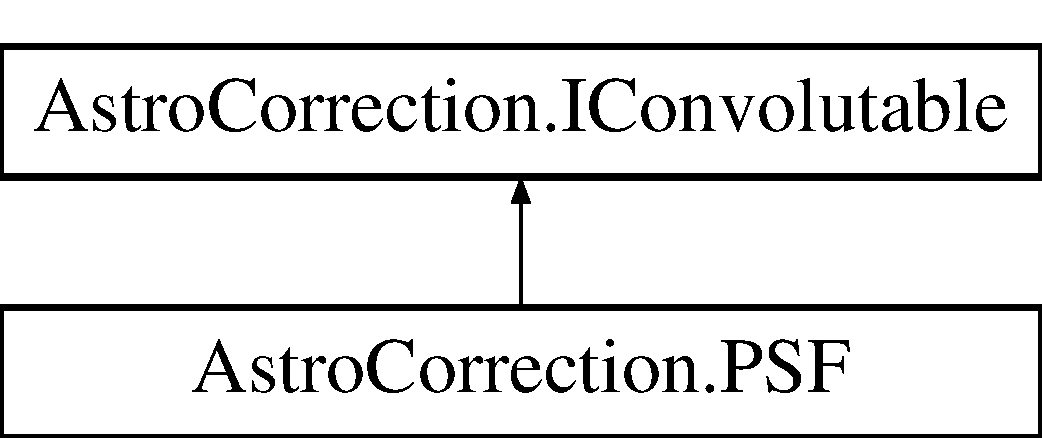
\includegraphics[height=2cm]{class_astro_correction_1_1_p_s_f}
\end{center}
\end{figure}
\subsection*{Public Member Functions}
\begin{DoxyCompactItemize}
\item 
void {\bf Normalize} ()
\item 
{\bf ImageF} {\bf Convolute} ({\bf ImageF} image)
\begin{DoxyCompactList}\small\item\em Convolute the object with the \doxyref{ImageF}{p.}{class_astro_correction_1_1_image_f}. \item\end{DoxyCompactList}\end{DoxyCompactItemize}
\subsection*{Static Public Member Functions}
\begin{DoxyCompactItemize}
\item 
static unsafe {\bf PSF} {\bf FromBitmap} ({\bf ImageF} image, Point pos)
\end{DoxyCompactItemize}
\subsection*{Properties}
\begin{DoxyCompactItemize}
\item 
Bitmap {\bf Bitmap}\hspace{0.3cm}{\ttfamily  [get]}
\item 
int {\bf Xmin}\hspace{0.3cm}{\ttfamily  [get, set]}
\item 
int {\bf Xmax}\hspace{0.3cm}{\ttfamily  [get, set]}
\item 
int {\bf Ymin}\hspace{0.3cm}{\ttfamily  [get, set]}
\item 
int {\bf Ymax}\hspace{0.3cm}{\ttfamily  [get, set]}
\item 
double {\bf this} [int x, int y]\hspace{0.3cm}{\ttfamily  [get, set]}
\end{DoxyCompactItemize}


\subsection{Detailed Description}
PixelData Spread Function. 

Definition at line 14 of file PSF.cs.

\subsection{Member Function Documentation}
\index{AstroCorrection::PSF@{AstroCorrection::PSF}!Convolute@{Convolute}}
\index{Convolute@{Convolute}!AstroCorrection::PSF@{AstroCorrection::PSF}}
\subsubsection[{Convolute}]{\setlength{\rightskip}{0pt plus 5cm}{\bf ImageF} AstroCorrection.PSF.Convolute ({\bf ImageF} {\em image})}\label{class_astro_correction_1_1_p_s_f_a81fbd1fefd705253807d8edc6502fed0}


Convolute the object with the \doxyref{ImageF}{p.}{class_astro_correction_1_1_image_f}. 
\begin{DoxyParams}{Parameters}
\item[{\em image}]The image to convolute with\end{DoxyParams}
\begin{DoxyReturn}{Returns}
The result of the convlution 
\end{DoxyReturn}


Implements {\bf AstroCorrection.IConvolutable} \doxyref{}{p.}{interface_astro_correction_1_1_i_convolutable_a01a503ab4927505350bc1865d4b8dd35}.

Definition at line 430 of file PSF.cs.\index{AstroCorrection::PSF@{AstroCorrection::PSF}!FromBitmap@{FromBitmap}}
\index{FromBitmap@{FromBitmap}!AstroCorrection::PSF@{AstroCorrection::PSF}}
\subsubsection[{FromBitmap}]{\setlength{\rightskip}{0pt plus 5cm}static unsafe {\bf PSF} AstroCorrection.PSF.FromBitmap ({\bf ImageF} {\em image}, \/  Point {\em pos})\hspace{0.3cm}{\ttfamily  [static]}}\label{class_astro_correction_1_1_p_s_f_a409f4a423853d4eb0b7acaabb946903f}


Definition at line 350 of file PSF.cs.\index{AstroCorrection::PSF@{AstroCorrection::PSF}!Normalize@{Normalize}}
\index{Normalize@{Normalize}!AstroCorrection::PSF@{AstroCorrection::PSF}}
\subsubsection[{Normalize}]{\setlength{\rightskip}{0pt plus 5cm}void AstroCorrection.PSF.Normalize ()}\label{class_astro_correction_1_1_p_s_f_ae2cb282db33d35a4ea09c7a291a9af74}


Definition at line 301 of file PSF.cs.

\subsection{Property Documentation}
\index{AstroCorrection::PSF@{AstroCorrection::PSF}!Bitmap@{Bitmap}}
\index{Bitmap@{Bitmap}!AstroCorrection::PSF@{AstroCorrection::PSF}}
\subsubsection[{Bitmap}]{\setlength{\rightskip}{0pt plus 5cm}Bitmap AstroCorrection.PSF.Bitmap\hspace{0.3cm}{\ttfamily  [get]}}\label{class_astro_correction_1_1_p_s_f_adfef23f1296ff43ec77c75aee9c719be}


Definition at line 19 of file PSF.cs.\index{AstroCorrection::PSF@{AstroCorrection::PSF}!this@{this}}
\index{this@{this}!AstroCorrection::PSF@{AstroCorrection::PSF}}
\subsubsection[{this}]{\setlength{\rightskip}{0pt plus 5cm}double AstroCorrection.PSF.this[int x, int y]\hspace{0.3cm}{\ttfamily  [get, set]}}\label{class_astro_correction_1_1_p_s_f_a30257a589239e6769f7e1fe2326692ef}


Definition at line 261 of file PSF.cs.\index{AstroCorrection::PSF@{AstroCorrection::PSF}!Xmax@{Xmax}}
\index{Xmax@{Xmax}!AstroCorrection::PSF@{AstroCorrection::PSF}}
\subsubsection[{Xmax}]{\setlength{\rightskip}{0pt plus 5cm}int AstroCorrection.PSF.Xmax\hspace{0.3cm}{\ttfamily  [get, set]}}\label{class_astro_correction_1_1_p_s_f_ae2ec7dbec5106d7f3e2e8929ab82af36}


Definition at line 87 of file PSF.cs.\index{AstroCorrection::PSF@{AstroCorrection::PSF}!Xmin@{Xmin}}
\index{Xmin@{Xmin}!AstroCorrection::PSF@{AstroCorrection::PSF}}
\subsubsection[{Xmin}]{\setlength{\rightskip}{0pt plus 5cm}int AstroCorrection.PSF.Xmin\hspace{0.3cm}{\ttfamily  [get, set]}}\label{class_astro_correction_1_1_p_s_f_a9159673400b8146f197d1f44c33342f0}


Definition at line 60 of file PSF.cs.\index{AstroCorrection::PSF@{AstroCorrection::PSF}!Ymax@{Ymax}}
\index{Ymax@{Ymax}!AstroCorrection::PSF@{AstroCorrection::PSF}}
\subsubsection[{Ymax}]{\setlength{\rightskip}{0pt plus 5cm}int AstroCorrection.PSF.Ymax\hspace{0.3cm}{\ttfamily  [get, set]}}\label{class_astro_correction_1_1_p_s_f_a4b5f3294e0c1eb96d948260465202f29}


Definition at line 137 of file PSF.cs.\index{AstroCorrection::PSF@{AstroCorrection::PSF}!Ymin@{Ymin}}
\index{Ymin@{Ymin}!AstroCorrection::PSF@{AstroCorrection::PSF}}
\subsubsection[{Ymin}]{\setlength{\rightskip}{0pt plus 5cm}int AstroCorrection.PSF.Ymin\hspace{0.3cm}{\ttfamily  [get, set]}}\label{class_astro_correction_1_1_p_s_f_a7b7b3af871822c340e1b293ede491e3d}


Definition at line 112 of file PSF.cs.

The documentation for this class was generated from the following file:\begin{DoxyCompactItemize}
\item 
C:/Users/Joost/Documents/Development/MyProjects/AstroCorrection/AstroCorrection/{\bf PSF.cs}\end{DoxyCompactItemize}

\section{AstroCorrection.PsfWrapper Class Reference}
\label{class_astro_correction_1_1_psf_wrapper}\index{AstroCorrection::PsfWrapper@{AstroCorrection::PsfWrapper}}
\subsection*{Public Member Functions}
\begin{DoxyCompactItemize}
\item 
{\bf PsfWrapper} ({\bf PSF} aPsf, Point aPosition)
\end{DoxyCompactItemize}
\subsection*{Properties}
\begin{DoxyCompactItemize}
\item 
Point {\bf Position}\hspace{0.3cm}{\ttfamily  [get, set]}
\item 
{\bf PSF} {\bf Psf}\hspace{0.3cm}{\ttfamily  [get, set]}
\end{DoxyCompactItemize}


\subsection{Detailed Description}
Wrapper around Point Spread Functions

Mostly used to serialize the \doxyref{PSF}{p.}{class_astro_correction_1_1_p_s_f} 

Definition at line 15 of file PsfWrapper.cs.

\subsection{Constructor \& Destructor Documentation}
\index{AstroCorrection::PsfWrapper@{AstroCorrection::PsfWrapper}!PsfWrapper@{PsfWrapper}}
\index{PsfWrapper@{PsfWrapper}!AstroCorrection::PsfWrapper@{AstroCorrection::PsfWrapper}}
\subsubsection[{PsfWrapper}]{\setlength{\rightskip}{0pt plus 5cm}AstroCorrection.PsfWrapper.PsfWrapper ({\bf PSF} {\em aPsf}, \/  Point {\em aPosition})}\label{class_astro_correction_1_1_psf_wrapper_a86df48ff477fb5be293e706a38d63432}
Constructor


\begin{DoxyParams}{Parameters}
\item[{\em aPsf}]The \doxyref{PSF}{p.}{class_astro_correction_1_1_p_s_f}\item[{\em aPosition}]The position of the \doxyref{PSF}{p.}{class_astro_correction_1_1_p_s_f} in the underlying picture \end{DoxyParams}


Definition at line 44 of file PsfWrapper.cs.

\subsection{Property Documentation}
\index{AstroCorrection::PsfWrapper@{AstroCorrection::PsfWrapper}!Position@{Position}}
\index{Position@{Position}!AstroCorrection::PsfWrapper@{AstroCorrection::PsfWrapper}}
\subsubsection[{Position}]{\setlength{\rightskip}{0pt plus 5cm}Point AstroCorrection.PsfWrapper.Position\hspace{0.3cm}{\ttfamily  [get, set]}}\label{class_astro_correction_1_1_psf_wrapper_a8002c5e312bfff068ccadacca3b43ca5}
The position of the center of the \doxyref{PSF}{p.}{class_astro_correction_1_1_p_s_f} 

Definition at line 21 of file PsfWrapper.cs.\index{AstroCorrection::PsfWrapper@{AstroCorrection::PsfWrapper}!Psf@{Psf}}
\index{Psf@{Psf}!AstroCorrection::PsfWrapper@{AstroCorrection::PsfWrapper}}
\subsubsection[{Psf}]{\setlength{\rightskip}{0pt plus 5cm}{\bf PSF} AstroCorrection.PsfWrapper.Psf\hspace{0.3cm}{\ttfamily  [get, set]}}\label{class_astro_correction_1_1_psf_wrapper_a31e99002b1ccb2e6750c6976bca1162a}
The \doxyref{PSF}{p.}{class_astro_correction_1_1_p_s_f} being wrapped 

Definition at line 30 of file PsfWrapper.cs.

The documentation for this class was generated from the following file:\begin{DoxyCompactItemize}
\item 
C:/Users/Joost/Documents/Development/MyProjects/AstroCorrection/AstroCorrection/{\bf PsfWrapper.cs}\end{DoxyCompactItemize}

\section{AstroCorrection.Properties.Resources Class Reference}
\label{class_astro_correction_1_1_properties_1_1_resources}\index{AstroCorrection::Properties::Resources@{AstroCorrection::Properties::Resources}}


A strongly-\/typed resource class, for looking up localized strings, etc.  


\subsection{Detailed Description}
A strongly-\/typed resource class, for looking up localized strings, etc. 

Definition at line 25 of file Resources.Designer.cs.

The documentation for this class was generated from the following file:\begin{DoxyCompactItemize}
\item 
C:/Users/Joost/Documents/Development/MyProjects/AstroCorrection/AstroCorrection/Properties/{\bf Resources.Designer.cs}\end{DoxyCompactItemize}

\section{AstroCorrection.RichardsonLucyDeconvolution Class Reference}
\label{class_astro_correction_1_1_richardson_lucy_deconvolution}\index{AstroCorrection::RichardsonLucyDeconvolution@{AstroCorrection::RichardsonLucyDeconvolution}}


\subsection{Detailed Description}


Definition at line 67 of file RichardsonLucyDeconvolution.cs.

The documentation for this class was generated from the following file:\begin{DoxyCompactItemize}
\item 
C:/Users/Joost/Documents/Development/MyProjects/AstroCorrection/AstroCorrection/{\bf RichardsonLucyDeconvolution.cs}\end{DoxyCompactItemize}

\section{AstroCorrection.RunningAverage Class Reference}
\label{class_astro_correction_1_1_running_average}\index{AstroCorrection::RunningAverage@{AstroCorrection::RunningAverage}}
\subsection*{Public Member Functions}
\begin{DoxyCompactItemize}
\item 
{\bf RunningAverage} (int span)
\item 
double {\bf Add} (double x)
\end{DoxyCompactItemize}
\subsection*{Properties}
\begin{DoxyCompactItemize}
\item 
double {\bf Average}\hspace{0.3cm}{\ttfamily  [get]}
\end{DoxyCompactItemize}


\subsection{Detailed Description}


Definition at line 10 of file RunningAverage.cs.

\subsection{Constructor \& Destructor Documentation}
\index{AstroCorrection::RunningAverage@{AstroCorrection::RunningAverage}!RunningAverage@{RunningAverage}}
\index{RunningAverage@{RunningAverage}!AstroCorrection::RunningAverage@{AstroCorrection::RunningAverage}}
\subsubsection[{RunningAverage}]{\setlength{\rightskip}{0pt plus 5cm}AstroCorrection.RunningAverage.RunningAverage (int {\em span})}\label{class_astro_correction_1_1_running_average_a274a4e739c8b92098d45987afb139459}


Definition at line 27 of file RunningAverage.cs.

\subsection{Member Function Documentation}
\index{AstroCorrection::RunningAverage@{AstroCorrection::RunningAverage}!Add@{Add}}
\index{Add@{Add}!AstroCorrection::RunningAverage@{AstroCorrection::RunningAverage}}
\subsubsection[{Add}]{\setlength{\rightskip}{0pt plus 5cm}double AstroCorrection.RunningAverage.Add (double {\em x})}\label{class_astro_correction_1_1_running_average_acfcaf2ffa54301ff88aae527748efcec}


Definition at line 33 of file RunningAverage.cs.

\subsection{Property Documentation}
\index{AstroCorrection::RunningAverage@{AstroCorrection::RunningAverage}!Average@{Average}}
\index{Average@{Average}!AstroCorrection::RunningAverage@{AstroCorrection::RunningAverage}}
\subsubsection[{Average}]{\setlength{\rightskip}{0pt plus 5cm}double AstroCorrection.RunningAverage.Average\hspace{0.3cm}{\ttfamily  [get]}}\label{class_astro_correction_1_1_running_average_a0866748792b2f22fa72d35a06b407566}


Definition at line 21 of file RunningAverage.cs.

The documentation for this class was generated from the following file:\begin{DoxyCompactItemize}
\item 
C:/Users/Joost/Documents/Development/MyProjects/AstroCorrection/AstroCorrection/{\bf RunningAverage.cs}\end{DoxyCompactItemize}

\section{AstroCorrection.RunningCovariance Class Reference}
\label{class_astro_correction_1_1_running_covariance}\index{AstroCorrection::RunningCovariance@{AstroCorrection::RunningCovariance}}
\subsection*{Public Member Functions}
\begin{DoxyCompactItemize}
\item 
{\bf RunningCovariance} ()
\item 
void {\bf Add} (double x, double y)
\end{DoxyCompactItemize}
\subsection*{Properties}
\begin{DoxyCompactItemize}
\item 
double {\bf MeanX}\hspace{0.3cm}{\ttfamily  [get, set]}
\item 
double {\bf MeanY}\hspace{0.3cm}{\ttfamily  [get, set]}
\item 
double {\bf Covariance}\hspace{0.3cm}{\ttfamily  [get]}
\end{DoxyCompactItemize}


\subsection{Detailed Description}


Definition at line 13 of file RunningCovariance.cs.

\subsection{Constructor \& Destructor Documentation}
\index{AstroCorrection::RunningCovariance@{AstroCorrection::RunningCovariance}!RunningCovariance@{RunningCovariance}}
\index{RunningCovariance@{RunningCovariance}!AstroCorrection::RunningCovariance@{AstroCorrection::RunningCovariance}}
\subsubsection[{RunningCovariance}]{\setlength{\rightskip}{0pt plus 5cm}AstroCorrection.RunningCovariance.RunningCovariance ()}\label{class_astro_correction_1_1_running_covariance_a10d660cf17ee3ad8f52d45848585c0e1}


Definition at line 21 of file RunningCovariance.cs.

\subsection{Member Function Documentation}
\index{AstroCorrection::RunningCovariance@{AstroCorrection::RunningCovariance}!Add@{Add}}
\index{Add@{Add}!AstroCorrection::RunningCovariance@{AstroCorrection::RunningCovariance}}
\subsubsection[{Add}]{\setlength{\rightskip}{0pt plus 5cm}void AstroCorrection.RunningCovariance.Add (double {\em x}, \/  double {\em y})}\label{class_astro_correction_1_1_running_covariance_aedd3e1361351ec7299963ee8c5d81ee1}


Definition at line 64 of file RunningCovariance.cs.

\subsection{Property Documentation}
\index{AstroCorrection::RunningCovariance@{AstroCorrection::RunningCovariance}!Covariance@{Covariance}}
\index{Covariance@{Covariance}!AstroCorrection::RunningCovariance@{AstroCorrection::RunningCovariance}}
\subsubsection[{Covariance}]{\setlength{\rightskip}{0pt plus 5cm}double AstroCorrection.RunningCovariance.Covariance\hspace{0.3cm}{\ttfamily  [get]}}\label{class_astro_correction_1_1_running_covariance_a5a68ff6963573eafcdfdf5233a89846e}


Definition at line 38 of file RunningCovariance.cs.\index{AstroCorrection::RunningCovariance@{AstroCorrection::RunningCovariance}!MeanX@{MeanX}}
\index{MeanX@{MeanX}!AstroCorrection::RunningCovariance@{AstroCorrection::RunningCovariance}}
\subsubsection[{MeanX}]{\setlength{\rightskip}{0pt plus 5cm}double AstroCorrection.RunningCovariance.MeanX\hspace{0.3cm}{\ttfamily  [get, set]}}\label{class_astro_correction_1_1_running_covariance_aff4f44dc5068a5abe01f4babfaf5ee4d}


Definition at line 26 of file RunningCovariance.cs.\index{AstroCorrection::RunningCovariance@{AstroCorrection::RunningCovariance}!MeanY@{MeanY}}
\index{MeanY@{MeanY}!AstroCorrection::RunningCovariance@{AstroCorrection::RunningCovariance}}
\subsubsection[{MeanY}]{\setlength{\rightskip}{0pt plus 5cm}double AstroCorrection.RunningCovariance.MeanY\hspace{0.3cm}{\ttfamily  [get, set]}}\label{class_astro_correction_1_1_running_covariance_a6b1908501a842face78b11a3ecc15aba}


Definition at line 32 of file RunningCovariance.cs.

The documentation for this class was generated from the following file:\begin{DoxyCompactItemize}
\item 
C:/Users/Joost/Documents/Development/MyProjects/AstroCorrection/AstroCorrection/{\bf RunningCovariance.cs}\end{DoxyCompactItemize}

\section{AstroCorrection.RunningStatistics Class Reference}
\label{class_astro_correction_1_1_running_statistics}\index{AstroCorrection::RunningStatistics@{AstroCorrection::RunningStatistics}}
\subsection*{Public Member Functions}
\begin{DoxyCompactItemize}
\item 
{\bf RunningStatistics} (int span)
\item 
void {\bf Clear} (int span)
\item 
void {\bf Add} (double x)
\end{DoxyCompactItemize}
\subsection*{Properties}
\begin{DoxyCompactItemize}
\item 
double {\bf Variance}\hspace{0.3cm}{\ttfamily  [get]}
\item 
double {\bf Mean}\hspace{0.3cm}{\ttfamily  [get]}
\end{DoxyCompactItemize}


\subsection{Detailed Description}


Definition at line 10 of file RunningVariance.cs.

\subsection{Constructor \& Destructor Documentation}
\index{AstroCorrection::RunningStatistics@{AstroCorrection::RunningStatistics}!RunningStatistics@{RunningStatistics}}
\index{RunningStatistics@{RunningStatistics}!AstroCorrection::RunningStatistics@{AstroCorrection::RunningStatistics}}
\subsubsection[{RunningStatistics}]{\setlength{\rightskip}{0pt plus 5cm}AstroCorrection.RunningStatistics.RunningStatistics (int {\em span})}\label{class_astro_correction_1_1_running_statistics_a18877e6c262ce9f46f9c5fd4060399d2}


Definition at line 36 of file RunningVariance.cs.

\subsection{Member Function Documentation}
\index{AstroCorrection::RunningStatistics@{AstroCorrection::RunningStatistics}!Add@{Add}}
\index{Add@{Add}!AstroCorrection::RunningStatistics@{AstroCorrection::RunningStatistics}}
\subsubsection[{Add}]{\setlength{\rightskip}{0pt plus 5cm}void AstroCorrection.RunningStatistics.Add (double {\em x})}\label{class_astro_correction_1_1_running_statistics_a7cc4df707d614b53d81d4610a11081c5}


Definition at line 49 of file RunningVariance.cs.\index{AstroCorrection::RunningStatistics@{AstroCorrection::RunningStatistics}!Clear@{Clear}}
\index{Clear@{Clear}!AstroCorrection::RunningStatistics@{AstroCorrection::RunningStatistics}}
\subsubsection[{Clear}]{\setlength{\rightskip}{0pt plus 5cm}void AstroCorrection.RunningStatistics.Clear (int {\em span})}\label{class_astro_correction_1_1_running_statistics_a9831f68e30b4c2c4213663d64087f552}


Definition at line 41 of file RunningVariance.cs.

\subsection{Property Documentation}
\index{AstroCorrection::RunningStatistics@{AstroCorrection::RunningStatistics}!Mean@{Mean}}
\index{Mean@{Mean}!AstroCorrection::RunningStatistics@{AstroCorrection::RunningStatistics}}
\subsubsection[{Mean}]{\setlength{\rightskip}{0pt plus 5cm}double AstroCorrection.RunningStatistics.Mean\hspace{0.3cm}{\ttfamily  [get]}}\label{class_astro_correction_1_1_running_statistics_a48e7d26e5f7e7c6b4b28d5be4aa87060}


Definition at line 29 of file RunningVariance.cs.\index{AstroCorrection::RunningStatistics@{AstroCorrection::RunningStatistics}!Variance@{Variance}}
\index{Variance@{Variance}!AstroCorrection::RunningStatistics@{AstroCorrection::RunningStatistics}}
\subsubsection[{Variance}]{\setlength{\rightskip}{0pt plus 5cm}double AstroCorrection.RunningStatistics.Variance\hspace{0.3cm}{\ttfamily  [get]}}\label{class_astro_correction_1_1_running_statistics_a86140be351d78a7b5ce75232ba630d4c}


Definition at line 22 of file RunningVariance.cs.

The documentation for this class was generated from the following file:\begin{DoxyCompactItemize}
\item 
C:/Users/Joost/Documents/Development/MyProjects/AstroCorrection/AstroCorrection/{\bf RunningVariance.cs}\end{DoxyCompactItemize}

\section{AstroCorrection.ScanLineAnalyzer Class Reference}
\label{class_astro_correction_1_1_scan_line_analyzer}\index{AstroCorrection::ScanLineAnalyzer@{AstroCorrection::ScanLineAnalyzer}}


Analyze a small piece of an image along a scan line (horizontal).  
\subsection*{Public Member Functions}
\begin{DoxyCompactItemize}
\item 
{\bf ScanLineAnalyzer} ({\bf ImageF} image, int scanLine, int xCenter)
\begin{DoxyCompactList}\small\item\em Constructor. \item\end{DoxyCompactList}\item 
{\bf ScanLineAnalyzer} ({\bf ImageF} image, int scanLine)
\item 
{\bf ScanLineAnalyzer} ({\bf ImageF} image)
\item 
void {\bf Analyze} (int xCenter, int scanLine)
\item 
void {\bf Analyze} (int xCenter)
\item 
bool {\bf FindBackground} ()
\item 
void {\bf Analyze} ()
\begin{DoxyCompactList}\small\item\em Analyze the scanline Scanline around point XCenter. \item\end{DoxyCompactList}\end{DoxyCompactItemize}
\subsection*{Properties}
\begin{DoxyCompactItemize}
\item 
int {\bf ScanLine}\hspace{0.3cm}{\ttfamily  [get, set]}
\begin{DoxyCompactList}\small\item\em The scanline being analyzed. \item\end{DoxyCompactList}\item 
int {\bf XCenter}\hspace{0.3cm}{\ttfamily  [get, set]}
\begin{DoxyCompactList}\small\item\em The X-\/coordinate along the scanline where the analysis starts. \item\end{DoxyCompactList}\item 
int {\bf LeftBackgroundPosition}\hspace{0.3cm}{\ttfamily  [get, set]}
\item 
double {\bf LeftBackground}\hspace{0.3cm}{\ttfamily  [get, set]}
\item 
double {\bf LeftBackgroundDeviation}\hspace{0.3cm}{\ttfamily  [get, set]}
\item 
int {\bf RightBackgroundPosition}\hspace{0.3cm}{\ttfamily  [get, set]}
\item 
double {\bf RightBackground}\hspace{0.3cm}{\ttfamily  [get, set]}
\item 
double {\bf RightBackgroundDeviation}\hspace{0.3cm}{\ttfamily  [get, set]}
\item 
bool {\bf IsBackgroundLine}\hspace{0.3cm}{\ttfamily  [get, set]}
\end{DoxyCompactItemize}


\subsection{Detailed Description}
Analyze a small piece of an image along a scan line (horizontal). 

Definition at line 11 of file ScanLineAnalyzer.cs.

\subsection{Constructor \& Destructor Documentation}
\index{AstroCorrection::ScanLineAnalyzer@{AstroCorrection::ScanLineAnalyzer}!ScanLineAnalyzer@{ScanLineAnalyzer}}
\index{ScanLineAnalyzer@{ScanLineAnalyzer}!AstroCorrection::ScanLineAnalyzer@{AstroCorrection::ScanLineAnalyzer}}
\subsubsection[{ScanLineAnalyzer}]{\setlength{\rightskip}{0pt plus 5cm}AstroCorrection.ScanLineAnalyzer.ScanLineAnalyzer ({\bf ImageF} {\em image}, \/  int {\em scanLine}, \/  int {\em xCenter})}\label{class_astro_correction_1_1_scan_line_analyzer_a68be7616e111fe6dfe4e51dcff8bd282}


Constructor. 
\begin{DoxyParams}{Parameters}
\item[{\em image}]\item[{\em scanLine}]\item[{\em xCenter}]\end{DoxyParams}


Definition at line 81 of file ScanLineAnalyzer.cs.\index{AstroCorrection::ScanLineAnalyzer@{AstroCorrection::ScanLineAnalyzer}!ScanLineAnalyzer@{ScanLineAnalyzer}}
\index{ScanLineAnalyzer@{ScanLineAnalyzer}!AstroCorrection::ScanLineAnalyzer@{AstroCorrection::ScanLineAnalyzer}}
\subsubsection[{ScanLineAnalyzer}]{\setlength{\rightskip}{0pt plus 5cm}AstroCorrection.ScanLineAnalyzer.ScanLineAnalyzer ({\bf ImageF} {\em image}, \/  int {\em scanLine})}\label{class_astro_correction_1_1_scan_line_analyzer_a244e89c43f71842f56190f1226b4df2b}


Definition at line 88 of file ScanLineAnalyzer.cs.\index{AstroCorrection::ScanLineAnalyzer@{AstroCorrection::ScanLineAnalyzer}!ScanLineAnalyzer@{ScanLineAnalyzer}}
\index{ScanLineAnalyzer@{ScanLineAnalyzer}!AstroCorrection::ScanLineAnalyzer@{AstroCorrection::ScanLineAnalyzer}}
\subsubsection[{ScanLineAnalyzer}]{\setlength{\rightskip}{0pt plus 5cm}AstroCorrection.ScanLineAnalyzer.ScanLineAnalyzer ({\bf ImageF} {\em image})}\label{class_astro_correction_1_1_scan_line_analyzer_a17ebcdc7b7d69ce60e32df2d55c9ba01}


Definition at line 94 of file ScanLineAnalyzer.cs.

\subsection{Member Function Documentation}
\index{AstroCorrection::ScanLineAnalyzer@{AstroCorrection::ScanLineAnalyzer}!Analyze@{Analyze}}
\index{Analyze@{Analyze}!AstroCorrection::ScanLineAnalyzer@{AstroCorrection::ScanLineAnalyzer}}
\subsubsection[{Analyze}]{\setlength{\rightskip}{0pt plus 5cm}void AstroCorrection.ScanLineAnalyzer.Analyze ()}\label{class_astro_correction_1_1_scan_line_analyzer_acb18e449588661b82dfbe7cc95d6788d}


Analyze the scanline Scanline around point XCenter. 

Definition at line 169 of file ScanLineAnalyzer.cs.\index{AstroCorrection::ScanLineAnalyzer@{AstroCorrection::ScanLineAnalyzer}!Analyze@{Analyze}}
\index{Analyze@{Analyze}!AstroCorrection::ScanLineAnalyzer@{AstroCorrection::ScanLineAnalyzer}}
\subsubsection[{Analyze}]{\setlength{\rightskip}{0pt plus 5cm}void AstroCorrection.ScanLineAnalyzer.Analyze (int {\em xCenter})}\label{class_astro_correction_1_1_scan_line_analyzer_a18201fcb160d0c1ff25ed1e0a6ebcb7b}


Definition at line 106 of file ScanLineAnalyzer.cs.\index{AstroCorrection::ScanLineAnalyzer@{AstroCorrection::ScanLineAnalyzer}!Analyze@{Analyze}}
\index{Analyze@{Analyze}!AstroCorrection::ScanLineAnalyzer@{AstroCorrection::ScanLineAnalyzer}}
\subsubsection[{Analyze}]{\setlength{\rightskip}{0pt plus 5cm}void AstroCorrection.ScanLineAnalyzer.Analyze (int {\em xCenter}, \/  int {\em scanLine})}\label{class_astro_correction_1_1_scan_line_analyzer_a18a0c0aa491c15ab2951b0ef2d5dfd50}


Definition at line 99 of file ScanLineAnalyzer.cs.\index{AstroCorrection::ScanLineAnalyzer@{AstroCorrection::ScanLineAnalyzer}!FindBackground@{FindBackground}}
\index{FindBackground@{FindBackground}!AstroCorrection::ScanLineAnalyzer@{AstroCorrection::ScanLineAnalyzer}}
\subsubsection[{FindBackground}]{\setlength{\rightskip}{0pt plus 5cm}bool AstroCorrection.ScanLineAnalyzer.FindBackground ()}\label{class_astro_correction_1_1_scan_line_analyzer_a9c85404e448688e43d6acf3a3908475b}


Definition at line 112 of file ScanLineAnalyzer.cs.

\subsection{Property Documentation}
\index{AstroCorrection::ScanLineAnalyzer@{AstroCorrection::ScanLineAnalyzer}!IsBackgroundLine@{IsBackgroundLine}}
\index{IsBackgroundLine@{IsBackgroundLine}!AstroCorrection::ScanLineAnalyzer@{AstroCorrection::ScanLineAnalyzer}}
\subsubsection[{IsBackgroundLine}]{\setlength{\rightskip}{0pt plus 5cm}bool AstroCorrection.ScanLineAnalyzer.IsBackgroundLine\hspace{0.3cm}{\ttfamily  [get, set]}}\label{class_astro_correction_1_1_scan_line_analyzer_abcdfd0525bbbd9e2cc6ee5229faf3240}


Definition at line 70 of file ScanLineAnalyzer.cs.\index{AstroCorrection::ScanLineAnalyzer@{AstroCorrection::ScanLineAnalyzer}!LeftBackground@{LeftBackground}}
\index{LeftBackground@{LeftBackground}!AstroCorrection::ScanLineAnalyzer@{AstroCorrection::ScanLineAnalyzer}}
\subsubsection[{LeftBackground}]{\setlength{\rightskip}{0pt plus 5cm}double AstroCorrection.ScanLineAnalyzer.LeftBackground\hspace{0.3cm}{\ttfamily  [get, set]}}\label{class_astro_correction_1_1_scan_line_analyzer_a7cc6965e905206faa71810054883d241}


Definition at line 44 of file ScanLineAnalyzer.cs.\index{AstroCorrection::ScanLineAnalyzer@{AstroCorrection::ScanLineAnalyzer}!LeftBackgroundDeviation@{LeftBackgroundDeviation}}
\index{LeftBackgroundDeviation@{LeftBackgroundDeviation}!AstroCorrection::ScanLineAnalyzer@{AstroCorrection::ScanLineAnalyzer}}
\subsubsection[{LeftBackgroundDeviation}]{\setlength{\rightskip}{0pt plus 5cm}double AstroCorrection.ScanLineAnalyzer.LeftBackgroundDeviation\hspace{0.3cm}{\ttfamily  [get, set]}}\label{class_astro_correction_1_1_scan_line_analyzer_afa03e0b3224363e5947b8a20f628187b}


Definition at line 49 of file ScanLineAnalyzer.cs.\index{AstroCorrection::ScanLineAnalyzer@{AstroCorrection::ScanLineAnalyzer}!LeftBackgroundPosition@{LeftBackgroundPosition}}
\index{LeftBackgroundPosition@{LeftBackgroundPosition}!AstroCorrection::ScanLineAnalyzer@{AstroCorrection::ScanLineAnalyzer}}
\subsubsection[{LeftBackgroundPosition}]{\setlength{\rightskip}{0pt plus 5cm}int AstroCorrection.ScanLineAnalyzer.LeftBackgroundPosition\hspace{0.3cm}{\ttfamily  [get, set]}}\label{class_astro_correction_1_1_scan_line_analyzer_acdb3b5a53b43635f60d1d9b62504421b}


Definition at line 39 of file ScanLineAnalyzer.cs.\index{AstroCorrection::ScanLineAnalyzer@{AstroCorrection::ScanLineAnalyzer}!RightBackground@{RightBackground}}
\index{RightBackground@{RightBackground}!AstroCorrection::ScanLineAnalyzer@{AstroCorrection::ScanLineAnalyzer}}
\subsubsection[{RightBackground}]{\setlength{\rightskip}{0pt plus 5cm}double AstroCorrection.ScanLineAnalyzer.RightBackground\hspace{0.3cm}{\ttfamily  [get, set]}}\label{class_astro_correction_1_1_scan_line_analyzer_adf22b766a041852a39004a36a38d35b9}


Definition at line 59 of file ScanLineAnalyzer.cs.\index{AstroCorrection::ScanLineAnalyzer@{AstroCorrection::ScanLineAnalyzer}!RightBackgroundDeviation@{RightBackgroundDeviation}}
\index{RightBackgroundDeviation@{RightBackgroundDeviation}!AstroCorrection::ScanLineAnalyzer@{AstroCorrection::ScanLineAnalyzer}}
\subsubsection[{RightBackgroundDeviation}]{\setlength{\rightskip}{0pt plus 5cm}double AstroCorrection.ScanLineAnalyzer.RightBackgroundDeviation\hspace{0.3cm}{\ttfamily  [get, set]}}\label{class_astro_correction_1_1_scan_line_analyzer_afddc7b114af358acc0aa5fca2ea5e0ca}


Definition at line 64 of file ScanLineAnalyzer.cs.\index{AstroCorrection::ScanLineAnalyzer@{AstroCorrection::ScanLineAnalyzer}!RightBackgroundPosition@{RightBackgroundPosition}}
\index{RightBackgroundPosition@{RightBackgroundPosition}!AstroCorrection::ScanLineAnalyzer@{AstroCorrection::ScanLineAnalyzer}}
\subsubsection[{RightBackgroundPosition}]{\setlength{\rightskip}{0pt plus 5cm}int AstroCorrection.ScanLineAnalyzer.RightBackgroundPosition\hspace{0.3cm}{\ttfamily  [get, set]}}\label{class_astro_correction_1_1_scan_line_analyzer_a8946b4fd40479263e925957cbd7b07fb}


Definition at line 54 of file ScanLineAnalyzer.cs.\index{AstroCorrection::ScanLineAnalyzer@{AstroCorrection::ScanLineAnalyzer}!ScanLine@{ScanLine}}
\index{ScanLine@{ScanLine}!AstroCorrection::ScanLineAnalyzer@{AstroCorrection::ScanLineAnalyzer}}
\subsubsection[{ScanLine}]{\setlength{\rightskip}{0pt plus 5cm}int AstroCorrection.ScanLineAnalyzer.ScanLine\hspace{0.3cm}{\ttfamily  [get, set]}}\label{class_astro_correction_1_1_scan_line_analyzer_a24a61483196c3193cb5ee42141139471}


The scanline being analyzed. 

Definition at line 24 of file ScanLineAnalyzer.cs.\index{AstroCorrection::ScanLineAnalyzer@{AstroCorrection::ScanLineAnalyzer}!XCenter@{XCenter}}
\index{XCenter@{XCenter}!AstroCorrection::ScanLineAnalyzer@{AstroCorrection::ScanLineAnalyzer}}
\subsubsection[{XCenter}]{\setlength{\rightskip}{0pt plus 5cm}int AstroCorrection.ScanLineAnalyzer.XCenter\hspace{0.3cm}{\ttfamily  [get, set]}}\label{class_astro_correction_1_1_scan_line_analyzer_ab54b1a23763c388577b1f07cbfb0c07d}


The X-\/coordinate along the scanline where the analysis starts. 

Definition at line 33 of file ScanLineAnalyzer.cs.

The documentation for this class was generated from the following file:\begin{DoxyCompactItemize}
\item 
C:/Users/Joost/Documents/Development/MyProjects/AstroCorrection/AstroCorrection/{\bf ScanLineAnalyzer.cs}\end{DoxyCompactItemize}

\section{AstroCorrection.SelectablePictureBox Class Reference}
\label{class_astro_correction_1_1_selectable_picture_box}\index{AstroCorrection::SelectablePictureBox@{AstroCorrection::SelectablePictureBox}}
\subsection*{Public Member Functions}
\begin{DoxyCompactItemize}
\item 
{\bf SelectablePictureBox} ()
\end{DoxyCompactItemize}
\subsection*{Protected Member Functions}
\begin{DoxyCompactItemize}
\item 
override void {\bf OnMouseDown} (MouseEventArgs e)
\item 
override void {\bf OnKeyPress} (KeyPressEventArgs e)
\item 
override void {\bf OnEnter} (EventArgs e)
\item 
override void {\bf OnLeave} (EventArgs e)
\item 
override void {\bf OnPaint} (PaintEventArgs pe)
\end{DoxyCompactItemize}


\subsection{Detailed Description}


Definition at line 10 of file SelectablePictureBox.cs.

\subsection{Constructor \& Destructor Documentation}
\index{AstroCorrection::SelectablePictureBox@{AstroCorrection::SelectablePictureBox}!SelectablePictureBox@{SelectablePictureBox}}
\index{SelectablePictureBox@{SelectablePictureBox}!AstroCorrection::SelectablePictureBox@{AstroCorrection::SelectablePictureBox}}
\subsubsection[{SelectablePictureBox}]{\setlength{\rightskip}{0pt plus 5cm}AstroCorrection.SelectablePictureBox.SelectablePictureBox ()}\label{class_astro_correction_1_1_selectable_picture_box_ae14f3d114a9f40b1e74ade813fc8ef0e}


Definition at line 12 of file SelectablePictureBox.cs.

\subsection{Member Function Documentation}
\index{AstroCorrection::SelectablePictureBox@{AstroCorrection::SelectablePictureBox}!OnEnter@{OnEnter}}
\index{OnEnter@{OnEnter}!AstroCorrection::SelectablePictureBox@{AstroCorrection::SelectablePictureBox}}
\subsubsection[{OnEnter}]{\setlength{\rightskip}{0pt plus 5cm}override void AstroCorrection.SelectablePictureBox.OnEnter (EventArgs {\em e})\hspace{0.3cm}{\ttfamily  [protected]}}\label{class_astro_correction_1_1_selectable_picture_box_aa3a6d049a5e5ffa2ae66527fa749a9dd}


Definition at line 36 of file SelectablePictureBox.cs.\index{AstroCorrection::SelectablePictureBox@{AstroCorrection::SelectablePictureBox}!OnKeyPress@{OnKeyPress}}
\index{OnKeyPress@{OnKeyPress}!AstroCorrection::SelectablePictureBox@{AstroCorrection::SelectablePictureBox}}
\subsubsection[{OnKeyPress}]{\setlength{\rightskip}{0pt plus 5cm}override void AstroCorrection.SelectablePictureBox.OnKeyPress (KeyPressEventArgs {\em e})\hspace{0.3cm}{\ttfamily  [protected]}}\label{class_astro_correction_1_1_selectable_picture_box_a074f15f2ca8610f57568ec3abe938243}


Definition at line 24 of file SelectablePictureBox.cs.\index{AstroCorrection::SelectablePictureBox@{AstroCorrection::SelectablePictureBox}!OnLeave@{OnLeave}}
\index{OnLeave@{OnLeave}!AstroCorrection::SelectablePictureBox@{AstroCorrection::SelectablePictureBox}}
\subsubsection[{OnLeave}]{\setlength{\rightskip}{0pt plus 5cm}override void AstroCorrection.SelectablePictureBox.OnLeave (EventArgs {\em e})\hspace{0.3cm}{\ttfamily  [protected]}}\label{class_astro_correction_1_1_selectable_picture_box_a47c19d77622a9ca8c3644f3d07187e6d}


Definition at line 42 of file SelectablePictureBox.cs.\index{AstroCorrection::SelectablePictureBox@{AstroCorrection::SelectablePictureBox}!OnMouseDown@{OnMouseDown}}
\index{OnMouseDown@{OnMouseDown}!AstroCorrection::SelectablePictureBox@{AstroCorrection::SelectablePictureBox}}
\subsubsection[{OnMouseDown}]{\setlength{\rightskip}{0pt plus 5cm}override void AstroCorrection.SelectablePictureBox.OnMouseDown (MouseEventArgs {\em e})\hspace{0.3cm}{\ttfamily  [protected]}}\label{class_astro_correction_1_1_selectable_picture_box_abcb24e54b36f17a31be3549cdf0abf69}


Definition at line 18 of file SelectablePictureBox.cs.\index{AstroCorrection::SelectablePictureBox@{AstroCorrection::SelectablePictureBox}!OnPaint@{OnPaint}}
\index{OnPaint@{OnPaint}!AstroCorrection::SelectablePictureBox@{AstroCorrection::SelectablePictureBox}}
\subsubsection[{OnPaint}]{\setlength{\rightskip}{0pt plus 5cm}override void AstroCorrection.SelectablePictureBox.OnPaint (PaintEventArgs {\em pe})\hspace{0.3cm}{\ttfamily  [protected]}}\label{class_astro_correction_1_1_selectable_picture_box_a3a34388b581990994a5ba41e136f7e9f}


Definition at line 48 of file SelectablePictureBox.cs.

The documentation for this class was generated from the following file:\begin{DoxyCompactItemize}
\item 
C:/Users/Joost/Documents/Development/MyProjects/AstroCorrection/AstroCorrection/{\bf SelectablePictureBox.cs}\end{DoxyCompactItemize}

\section{AstroCorrection.Properties.Settings Class Reference}
\label{class_astro_correction_1_1_properties_1_1_settings}\index{AstroCorrection::Properties::Settings@{AstroCorrection::Properties::Settings}}
\subsection*{Properties}
\begin{DoxyCompactItemize}
\item 
static {\bf Settings} {\bf Default}\hspace{0.3cm}{\ttfamily  [get]}
\end{DoxyCompactItemize}


\subsection{Detailed Description}


Definition at line 17 of file Settings.Designer.cs.

\subsection{Property Documentation}
\index{AstroCorrection::Properties::Settings@{AstroCorrection::Properties::Settings}!Default@{Default}}
\index{Default@{Default}!AstroCorrection::Properties::Settings@{AstroCorrection::Properties::Settings}}
\subsubsection[{Default}]{\setlength{\rightskip}{0pt plus 5cm}{\bf Settings} AstroCorrection.Properties.Settings.Default\hspace{0.3cm}{\ttfamily  [static, get]}}\label{class_astro_correction_1_1_properties_1_1_settings_a601b0a6c459a91ead39972a5873d042c}


Definition at line 23 of file Settings.Designer.cs.

The documentation for this class was generated from the following file:\begin{DoxyCompactItemize}
\item 
C:/Users/Joost/Documents/Development/MyProjects/AstroCorrection/AstroCorrection/Properties/{\bf Settings.Designer.cs}\end{DoxyCompactItemize}

\section{AstroCorrection.ShiftingArray$<$ T $>$ Class Template Reference}
\label{class_astro_correction_1_1_shifting_array_3_01_t_01_4}\index{AstroCorrection::ShiftingArray$<$ T $>$@{AstroCorrection::ShiftingArray$<$ T $>$}}
\subsection*{Public Member Functions}
\begin{DoxyCompactItemize}
\item 
{\bf ShiftingArray} (int size)
\item 
void {\bf Add} (T value)
\end{DoxyCompactItemize}
\subsection*{Properties}
\begin{DoxyCompactItemize}
\item 
int {\bf Span}\hspace{0.3cm}{\ttfamily  [get]}
\item 
T {\bf this} [int idx]\hspace{0.3cm}{\ttfamily  [get]}
\end{DoxyCompactItemize}


\subsection{Detailed Description}
\subsubsection*{template$<$T$>$ class AstroCorrection::ShiftingArray$<$ T $>$}



Definition at line 12 of file ShiftingArray.cs.

\subsection{Constructor \& Destructor Documentation}
\index{AstroCorrection::ShiftingArray$<$ T $>$@{AstroCorrection::ShiftingArray$<$ T $>$}!ShiftingArray@{ShiftingArray}}
\index{ShiftingArray@{ShiftingArray}!AstroCorrection::ShiftingArray< T >@{AstroCorrection::ShiftingArray$<$ T $>$}}
\subsubsection[{ShiftingArray}]{\setlength{\rightskip}{0pt plus 5cm}template$<$T $>$ AstroCorrection.ShiftingArray$<$ T $>$.ShiftingArray (int {\em size})}\label{class_astro_correction_1_1_shifting_array_3_01_t_01_4_a6bde97c87f3f2c33d906e280f54d9164}


Definition at line 30 of file ShiftingArray.cs.

\subsection{Member Function Documentation}
\index{AstroCorrection::ShiftingArray$<$ T $>$@{AstroCorrection::ShiftingArray$<$ T $>$}!Add@{Add}}
\index{Add@{Add}!AstroCorrection::ShiftingArray< T >@{AstroCorrection::ShiftingArray$<$ T $>$}}
\subsubsection[{Add}]{\setlength{\rightskip}{0pt plus 5cm}template$<$T $>$ void AstroCorrection.ShiftingArray$<$ T $>$.Add (T {\em value})}\label{class_astro_correction_1_1_shifting_array_3_01_t_01_4_a763fae5c8ea4db5576294ed297242c86}


Definition at line 35 of file ShiftingArray.cs.

\subsection{Property Documentation}
\index{AstroCorrection::ShiftingArray$<$ T $>$@{AstroCorrection::ShiftingArray$<$ T $>$}!Span@{Span}}
\index{Span@{Span}!AstroCorrection::ShiftingArray< T >@{AstroCorrection::ShiftingArray$<$ T $>$}}
\subsubsection[{Span}]{\setlength{\rightskip}{0pt plus 5cm}template$<$T $>$ int AstroCorrection.ShiftingArray$<$ T $>$.Span\hspace{0.3cm}{\ttfamily  [get]}}\label{class_astro_correction_1_1_shifting_array_3_01_t_01_4_a00a685bef0dbaa2437419119a0ffed09}


Definition at line 17 of file ShiftingArray.cs.\index{AstroCorrection::ShiftingArray$<$ T $>$@{AstroCorrection::ShiftingArray$<$ T $>$}!this@{this}}
\index{this@{this}!AstroCorrection::ShiftingArray< T >@{AstroCorrection::ShiftingArray$<$ T $>$}}
\subsubsection[{this}]{\setlength{\rightskip}{0pt plus 5cm}template$<$T $>$ T AstroCorrection.ShiftingArray$<$ T $>$.this[int idx]\hspace{0.3cm}{\ttfamily  [get]}}\label{class_astro_correction_1_1_shifting_array_3_01_t_01_4_a8cbba66e93d0b6255413ac109682dc73}


Definition at line 45 of file ShiftingArray.cs.

The documentation for this class was generated from the following file:\begin{DoxyCompactItemize}
\item 
C:/Users/Joost/Documents/Development/MyProjects/AstroCorrection/AstroCorrection/{\bf ShiftingArray.cs}\end{DoxyCompactItemize}

\chapter{File Documentation}
\section{C:/Users/Joost/Documents/Development/MyProjects/AstroCorrection/AstroCorrection/CompoundPSF.cs File Reference}
\label{_compound_p_s_f_8cs}\index{C:/Users/Joost/Documents/Development/MyProjects/AstroCorrection/AstroCorrection/CompoundPSF.cs@{C:/Users/Joost/Documents/Development/MyProjects/AstroCorrection/AstroCorrection/CompoundPSF.cs}}
\subsection*{Classes}
\begin{DoxyCompactItemize}
\item 
class {\bf AstroCorrection.CompoundPSF}
\begin{DoxyCompactList}\small\item\em Spatially Variant \doxyref{PSF}{p.}{class_astro_correction_1_1_p_s_f}, with Karhunen-\/Loève decomposition. \item\end{DoxyCompactList}\end{DoxyCompactItemize}
\subsection*{Packages}
\begin{DoxyCompactItemize}
\item 
package {\bf AstroCorrection}
\end{DoxyCompactItemize}
\subsection*{Variables}
\begin{DoxyCompactItemize}
\item 
using {\bf System}
\end{DoxyCompactItemize}


\subsection{Variable Documentation}
\index{CompoundPSF.cs@{CompoundPSF.cs}!System@{System}}
\index{System@{System}!CompoundPSF.cs@{CompoundPSF.cs}}
\subsubsection[{System}]{\setlength{\rightskip}{0pt plus 5cm}using {\bf System}}\label{_compound_p_s_f_8cs_a81a223a02c34d82b47199f08308847f2}


Definition at line 1 of file CompoundPSF.cs.
\section{C:/Users/Joost/Documents/Development/MyProjects/AstroCorrection/AstroCorrection/CovarianceBuilder.cs File Reference}
\label{_covariance_builder_8cs}\index{C:/Users/Joost/Documents/Development/MyProjects/AstroCorrection/AstroCorrection/CovarianceBuilder.cs@{C:/Users/Joost/Documents/Development/MyProjects/AstroCorrection/AstroCorrection/CovarianceBuilder.cs}}
\subsection*{Classes}
\begin{DoxyCompactItemize}
\item 
class {\bf AstroCorrection.CovarianceBuilder}
\end{DoxyCompactItemize}
\subsection*{Packages}
\begin{DoxyCompactItemize}
\item 
package {\bf AstroCorrection}
\end{DoxyCompactItemize}
\subsection*{Variables}
\begin{DoxyCompactItemize}
\item 
using {\bf System}
\end{DoxyCompactItemize}


\subsection{Variable Documentation}
\index{CovarianceBuilder.cs@{CovarianceBuilder.cs}!System@{System}}
\index{System@{System}!CovarianceBuilder.cs@{CovarianceBuilder.cs}}
\subsubsection[{System}]{\setlength{\rightskip}{0pt plus 5cm}using {\bf System}}\label{_covariance_builder_8cs_a81a223a02c34d82b47199f08308847f2}


Definition at line 1 of file CovarianceBuilder.cs.
\section{C:/Users/Joost/Documents/Development/MyProjects/AstroCorrection/AstroCorrection/HotellingTransform.cs File Reference}
\label{_hotelling_transform_8cs}\index{C:/Users/Joost/Documents/Development/MyProjects/AstroCorrection/AstroCorrection/HotellingTransform.cs@{C:/Users/Joost/Documents/Development/MyProjects/AstroCorrection/AstroCorrection/HotellingTransform.cs}}
\subsection*{Classes}
\begin{DoxyCompactItemize}
\item 
class {\bf AstroCorrection.HotellingTransform}
\item 
struct {\bfseries AstroCorrection.HotellingTransform.EigenElement}
\end{DoxyCompactItemize}
\subsection*{Packages}
\begin{DoxyCompactItemize}
\item 
package {\bf AstroCorrection}
\end{DoxyCompactItemize}
\subsection*{Variables}
\begin{DoxyCompactItemize}
\item 
using {\bf System}
\end{DoxyCompactItemize}


\subsection{Variable Documentation}
\index{HotellingTransform.cs@{HotellingTransform.cs}!System@{System}}
\index{System@{System}!HotellingTransform.cs@{HotellingTransform.cs}}
\subsubsection[{System}]{\setlength{\rightskip}{0pt plus 5cm}using {\bf System}}\label{_hotelling_transform_8cs_a81a223a02c34d82b47199f08308847f2}


Definition at line 1 of file HotellingTransform.cs.
\section{C:/Users/Joost/Documents/Development/MyProjects/AstroCorrection/AstroCorrection/IConvolutable.cs File Reference}
\label{_i_convolutable_8cs}\index{C:/Users/Joost/Documents/Development/MyProjects/AstroCorrection/AstroCorrection/IConvolutable.cs@{C:/Users/Joost/Documents/Development/MyProjects/AstroCorrection/AstroCorrection/IConvolutable.cs}}
\subsection*{Classes}
\begin{DoxyCompactItemize}
\item 
interface {\bf AstroCorrection.IConvolutable}
\begin{DoxyCompactList}\small\item\em Interface that allows Convolution into an \doxyref{ImageF}{p.}{class_astro_correction_1_1_image_f}. \item\end{DoxyCompactList}\end{DoxyCompactItemize}
\subsection*{Packages}
\begin{DoxyCompactItemize}
\item 
package {\bf AstroCorrection}
\end{DoxyCompactItemize}
\subsection*{Variables}
\begin{DoxyCompactItemize}
\item 
using {\bf System}
\end{DoxyCompactItemize}


\subsection{Variable Documentation}
\index{IConvolutable.cs@{IConvolutable.cs}!System@{System}}
\index{System@{System}!IConvolutable.cs@{IConvolutable.cs}}
\subsubsection[{System}]{\setlength{\rightskip}{0pt plus 5cm}using {\bf System}}\label{_i_convolutable_8cs_a81a223a02c34d82b47199f08308847f2}


Definition at line 1 of file IConvolutable.cs.
\section{C:/Users/Joost/Documents/Development/MyProjects/AstroCorrection/AstroCorrection/ImageF.cs File Reference}
\label{_image_f_8cs}\index{C:/Users/Joost/Documents/Development/MyProjects/AstroCorrection/AstroCorrection/ImageF.cs@{C:/Users/Joost/Documents/Development/MyProjects/AstroCorrection/AstroCorrection/ImageF.cs}}
\subsection*{Classes}
\begin{DoxyCompactItemize}
\item 
class {\bf AstroCorrection.ImageF}
\begin{DoxyCompactList}\small\item\em Monochrome image where the pixels are stored as floating point numbers. \item\end{DoxyCompactList}\end{DoxyCompactItemize}
\subsection*{Packages}
\begin{DoxyCompactItemize}
\item 
package {\bf AstroCorrection}
\end{DoxyCompactItemize}
\subsection*{Variables}
\begin{DoxyCompactItemize}
\item 
using {\bf System}
\end{DoxyCompactItemize}


\subsection{Variable Documentation}
\index{ImageF.cs@{ImageF.cs}!System@{System}}
\index{System@{System}!ImageF.cs@{ImageF.cs}}
\subsubsection[{System}]{\setlength{\rightskip}{0pt plus 5cm}using {\bf System}}\label{_image_f_8cs_a81a223a02c34d82b47199f08308847f2}


Definition at line 1 of file ImageF.cs.
\section{C:/Users/Joost/Documents/Development/MyProjects/AstroCorrection/AstroCorrection/ImageScan.cs File Reference}
\label{_image_scan_8cs}\index{C:/Users/Joost/Documents/Development/MyProjects/AstroCorrection/AstroCorrection/ImageScan.cs@{C:/Users/Joost/Documents/Development/MyProjects/AstroCorrection/AstroCorrection/ImageScan.cs}}
\subsection*{Classes}
\begin{DoxyCompactItemize}
\item 
class {\bf AstroCorrection.ImageScan}
\begin{DoxyCompactList}\small\item\em Show \doxyref{PSF}{p.}{class_astro_correction_1_1_p_s_f} images in a 'film strip'. \item\end{DoxyCompactList}\end{DoxyCompactItemize}
\subsection*{Packages}
\begin{DoxyCompactItemize}
\item 
package {\bf AstroCorrection}
\end{DoxyCompactItemize}
\subsection*{Variables}
\begin{DoxyCompactItemize}
\item 
using {\bf System}
\end{DoxyCompactItemize}


\subsection{Variable Documentation}
\index{ImageScan.cs@{ImageScan.cs}!System@{System}}
\index{System@{System}!ImageScan.cs@{ImageScan.cs}}
\subsubsection[{System}]{\setlength{\rightskip}{0pt plus 5cm}using {\bf System}}\label{_image_scan_8cs_a81a223a02c34d82b47199f08308847f2}


Definition at line 1 of file ImageScan.cs.
\section{C:/Users/Joost/Documents/Development/MyProjects/AstroCorrection/AstroCorrection/KLCoefficients.cs File Reference}
\label{_k_l_coefficients_8cs}\index{C:/Users/Joost/Documents/Development/MyProjects/AstroCorrection/AstroCorrection/KLCoefficients.cs@{C:/Users/Joost/Documents/Development/MyProjects/AstroCorrection/AstroCorrection/KLCoefficients.cs}}
\subsection*{Classes}
\begin{DoxyCompactItemize}
\item 
class {\bf AstroCorrection.KLCoefficients}
\begin{DoxyCompactList}\small\item\em Base class for Coefficients in Karhunen-\/Loève PSF decomposition. \item\end{DoxyCompactList}\end{DoxyCompactItemize}
\subsection*{Packages}
\begin{DoxyCompactItemize}
\item 
package {\bf AstroCorrection}
\end{DoxyCompactItemize}
\subsection*{Variables}
\begin{DoxyCompactItemize}
\item 
using {\bf System}
\end{DoxyCompactItemize}


\subsection{Variable Documentation}
\index{KLCoefficients.cs@{KLCoefficients.cs}!System@{System}}
\index{System@{System}!KLCoefficients.cs@{KLCoefficients.cs}}
\subsubsection[{System}]{\setlength{\rightskip}{0pt plus 5cm}using {\bf System}}\label{_k_l_coefficients_8cs_a81a223a02c34d82b47199f08308847f2}


Definition at line 1 of file KLCoefficients.cs.
\section{C:/Users/Joost/Documents/Development/MyProjects/AstroCorrection/AstroCorrection/MainForm.cs File Reference}
\label{_main_form_8cs}\index{C:/Users/Joost/Documents/Development/MyProjects/AstroCorrection/AstroCorrection/MainForm.cs@{C:/Users/Joost/Documents/Development/MyProjects/AstroCorrection/AstroCorrection/MainForm.cs}}
\subsection*{Classes}
\begin{DoxyCompactItemize}
\item 
class {\bf AstroCorrection.MainForm}
\end{DoxyCompactItemize}
\subsection*{Packages}
\begin{DoxyCompactItemize}
\item 
package {\bf AstroCorrection}
\end{DoxyCompactItemize}
\subsection*{Variables}
\begin{DoxyCompactItemize}
\item 
using {\bf System}
\end{DoxyCompactItemize}


\subsection{Variable Documentation}
\index{MainForm.cs@{MainForm.cs}!System@{System}}
\index{System@{System}!MainForm.cs@{MainForm.cs}}
\subsubsection[{System}]{\setlength{\rightskip}{0pt plus 5cm}using {\bf System}}\label{_main_form_8cs_a81a223a02c34d82b47199f08308847f2}


Definition at line 1 of file MainForm.cs.
\section{C:/Users/Joost/Documents/Development/MyProjects/AstroCorrection/AstroCorrection/MainForm.Designer.cs File Reference}
\label{_main_form_8_designer_8cs}\index{C:/Users/Joost/Documents/Development/MyProjects/AstroCorrection/AstroCorrection/MainForm.Designer.cs@{C:/Users/Joost/Documents/Development/MyProjects/AstroCorrection/AstroCorrection/MainForm.Designer.cs}}
\subsection*{Variables}
\begin{DoxyCompactItemize}
\item 
namespace {\bf AstroCorrection}
\end{DoxyCompactItemize}


\subsection{Variable Documentation}
\index{MainForm.Designer.cs@{MainForm.Designer.cs}!AstroCorrection@{AstroCorrection}}
\index{AstroCorrection@{AstroCorrection}!MainForm.Designer.cs@{MainForm.Designer.cs}}
\subsubsection[{AstroCorrection}]{\setlength{\rightskip}{0pt plus 5cm}namespace AstroCorrection}\label{_main_form_8_designer_8cs_ae380fdafc7c10e7ca4c67864e4f6f820}


Definition at line 2 of file MainForm.Designer.cs.
\section{C:/Users/Joost/Documents/Development/MyProjects/AstroCorrection/AstroCorrection/PhotographData.cs File Reference}
\label{_photograph_data_8cs}\index{C:/Users/Joost/Documents/Development/MyProjects/AstroCorrection/AstroCorrection/PhotographData.cs@{C:/Users/Joost/Documents/Development/MyProjects/AstroCorrection/AstroCorrection/PhotographData.cs}}
\subsection*{Classes}
\begin{DoxyCompactItemize}
\item 
class {\bf AstroCorrection.PhotographData}
\begin{DoxyCompactList}\small\item\em Wrapper around photograph data. \item\end{DoxyCompactList}\item 
struct {\bf AstroCorrection.PhotographData.PixelData}
\begin{DoxyCompactList}\small\item\em Data about a single pixel. \item\end{DoxyCompactList}\end{DoxyCompactItemize}
\subsection*{Packages}
\begin{DoxyCompactItemize}
\item 
package {\bf AstroCorrection}
\end{DoxyCompactItemize}
\subsection*{Variables}
\begin{DoxyCompactItemize}
\item 
using {\bf System}
\end{DoxyCompactItemize}


\subsection{Variable Documentation}
\index{PhotographData.cs@{PhotographData.cs}!System@{System}}
\index{System@{System}!PhotographData.cs@{PhotographData.cs}}
\subsubsection[{System}]{\setlength{\rightskip}{0pt plus 5cm}using {\bf System}}\label{_photograph_data_8cs_a81a223a02c34d82b47199f08308847f2}


Definition at line 1 of file PhotographData.cs.
\section{C:/Users/Joost/Documents/Development/MyProjects/AstroCorrection/AstroCorrection/Program.cs File Reference}
\label{_program_8cs}\index{C:/Users/Joost/Documents/Development/MyProjects/AstroCorrection/AstroCorrection/Program.cs@{C:/Users/Joost/Documents/Development/MyProjects/AstroCorrection/AstroCorrection/Program.cs}}
\subsection*{Classes}
\begin{DoxyCompactItemize}
\item 
class {\bfseries AstroCorrection.Program}
\end{DoxyCompactItemize}
\subsection*{Packages}
\begin{DoxyCompactItemize}
\item 
package {\bf AstroCorrection}
\end{DoxyCompactItemize}
\subsection*{Variables}
\begin{DoxyCompactItemize}
\item 
using {\bf System}
\end{DoxyCompactItemize}


\subsection{Variable Documentation}
\index{Program.cs@{Program.cs}!System@{System}}
\index{System@{System}!Program.cs@{Program.cs}}
\subsubsection[{System}]{\setlength{\rightskip}{0pt plus 5cm}using {\bf System}}\label{_program_8cs_a81a223a02c34d82b47199f08308847f2}


Definition at line 1 of file Program.cs.
\section{C:/Users/Joost/Documents/Development/MyProjects/AstroCorrection/AstroCorrection/Properties/AssemblyInfo.cs File Reference}
\label{_assembly_info_8cs}\index{C:/Users/Joost/Documents/Development/MyProjects/AstroCorrection/AstroCorrection/Properties/AssemblyInfo.cs@{C:/Users/Joost/Documents/Development/MyProjects/AstroCorrection/AstroCorrection/Properties/AssemblyInfo.cs}}
\subsection*{Variables}
\begin{DoxyCompactItemize}
\item 
using System. {\bf Reflection}
\end{DoxyCompactItemize}


\subsection{Variable Documentation}
\index{AssemblyInfo.cs@{AssemblyInfo.cs}!Reflection@{Reflection}}
\index{Reflection@{Reflection}!AssemblyInfo.cs@{AssemblyInfo.cs}}
\subsubsection[{Reflection}]{\setlength{\rightskip}{0pt plus 5cm}using System. {\bf Reflection}}\label{_assembly_info_8cs_a8974f59db973551affdb297a3c5ab53a}


Definition at line 1 of file AssemblyInfo.cs.
\section{C:/Users/Joost/Documents/Development/MyProjects/AstroCorrection/AstroCorrection/Properties/Resources.Designer.cs File Reference}
\label{_resources_8_designer_8cs}\index{C:/Users/Joost/Documents/Development/MyProjects/AstroCorrection/AstroCorrection/Properties/Resources.Designer.cs@{C:/Users/Joost/Documents/Development/MyProjects/AstroCorrection/AstroCorrection/Properties/Resources.Designer.cs}}
\subsection*{Classes}
\begin{DoxyCompactItemize}
\item 
class {\bf AstroCorrection.Properties.Resources}
\begin{DoxyCompactList}\small\item\em A strongly-\/typed resource class, for looking up localized strings, etc. \item\end{DoxyCompactList}\end{DoxyCompactItemize}
\subsection*{Packages}
\begin{DoxyCompactItemize}
\item 
package {\bf AstroCorrection.Properties}
\end{DoxyCompactItemize}

\section{C:/Users/Joost/Documents/Development/MyProjects/AstroCorrection/AstroCorrection/Properties/Settings.Designer.cs File Reference}
\label{_settings_8_designer_8cs}\index{C:/Users/Joost/Documents/Development/MyProjects/AstroCorrection/AstroCorrection/Properties/Settings.Designer.cs@{C:/Users/Joost/Documents/Development/MyProjects/AstroCorrection/AstroCorrection/Properties/Settings.Designer.cs}}
\subsection*{Classes}
\begin{DoxyCompactItemize}
\item 
class {\bf AstroCorrection.Properties.Settings}
\end{DoxyCompactItemize}
\subsection*{Packages}
\begin{DoxyCompactItemize}
\item 
package {\bf AstroCorrection.Properties}
\end{DoxyCompactItemize}

\section{C:/Users/Joost/Documents/Development/MyProjects/AstroCorrection/AstroCorrection/PSF.cs File Reference}
\label{_p_s_f_8cs}\index{C:/Users/Joost/Documents/Development/MyProjects/AstroCorrection/AstroCorrection/PSF.cs@{C:/Users/Joost/Documents/Development/MyProjects/AstroCorrection/AstroCorrection/PSF.cs}}
\subsection*{Classes}
\begin{DoxyCompactItemize}
\item 
class {\bf AstroCorrection.PSF}
\begin{DoxyCompactList}\small\item\em PixelData Spread Function. \item\end{DoxyCompactList}\end{DoxyCompactItemize}
\subsection*{Packages}
\begin{DoxyCompactItemize}
\item 
package {\bf AstroCorrection}
\end{DoxyCompactItemize}
\subsection*{Variables}
\begin{DoxyCompactItemize}
\item 
using {\bf System}
\end{DoxyCompactItemize}


\subsection{Variable Documentation}
\index{PSF.cs@{PSF.cs}!System@{System}}
\index{System@{System}!PSF.cs@{PSF.cs}}
\subsubsection[{System}]{\setlength{\rightskip}{0pt plus 5cm}using {\bf System}}\label{_p_s_f_8cs_a81a223a02c34d82b47199f08308847f2}


Definition at line 1 of file PSF.cs.
\section{C:/Users/Joost/Documents/Development/MyProjects/AstroCorrection/AstroCorrection/PsfWrapper.cs File Reference}
\label{_psf_wrapper_8cs}\index{C:/Users/Joost/Documents/Development/MyProjects/AstroCorrection/AstroCorrection/PsfWrapper.cs@{C:/Users/Joost/Documents/Development/MyProjects/AstroCorrection/AstroCorrection/PsfWrapper.cs}}
\subsection*{Classes}
\begin{DoxyCompactItemize}
\item 
class {\bf AstroCorrection.PsfWrapper}
\end{DoxyCompactItemize}
\subsection*{Packages}
\begin{DoxyCompactItemize}
\item 
package {\bf AstroCorrection}
\end{DoxyCompactItemize}
\subsection*{Variables}
\begin{DoxyCompactItemize}
\item 
using {\bf System}
\end{DoxyCompactItemize}


\subsection{Variable Documentation}
\index{PsfWrapper.cs@{PsfWrapper.cs}!System@{System}}
\index{System@{System}!PsfWrapper.cs@{PsfWrapper.cs}}
\subsubsection[{System}]{\setlength{\rightskip}{0pt plus 5cm}using {\bf System}}\label{_psf_wrapper_8cs_a81a223a02c34d82b47199f08308847f2}


Definition at line 1 of file PsfWrapper.cs.
\section{C:/Users/Joost/Documents/Development/MyProjects/AstroCorrection/AstroCorrection/RichardsonLucyDeconvolution.cs File Reference}
\label{_richardson_lucy_deconvolution_8cs}\index{C:/Users/Joost/Documents/Development/MyProjects/AstroCorrection/AstroCorrection/RichardsonLucyDeconvolution.cs@{C:/Users/Joost/Documents/Development/MyProjects/AstroCorrection/AstroCorrection/RichardsonLucyDeconvolution.cs}}
\subsection*{Classes}
\begin{DoxyCompactItemize}
\item 
class {\bf AstroCorrection.RichardsonLucyDeconvolution}
\end{DoxyCompactItemize}
\subsection*{Packages}
\begin{DoxyCompactItemize}
\item 
package {\bf AstroCorrection}
\end{DoxyCompactItemize}

\section{C:/Users/Joost/Documents/Development/MyProjects/AstroCorrection/AstroCorrection/RunningAverage.cs File Reference}
\label{_running_average_8cs}\index{C:/Users/Joost/Documents/Development/MyProjects/AstroCorrection/AstroCorrection/RunningAverage.cs@{C:/Users/Joost/Documents/Development/MyProjects/AstroCorrection/AstroCorrection/RunningAverage.cs}}
\subsection*{Classes}
\begin{DoxyCompactItemize}
\item 
class {\bf AstroCorrection.RunningAverage}
\end{DoxyCompactItemize}
\subsection*{Packages}
\begin{DoxyCompactItemize}
\item 
package {\bf AstroCorrection}
\end{DoxyCompactItemize}
\subsection*{Variables}
\begin{DoxyCompactItemize}
\item 
using {\bf System}
\end{DoxyCompactItemize}


\subsection{Variable Documentation}
\index{RunningAverage.cs@{RunningAverage.cs}!System@{System}}
\index{System@{System}!RunningAverage.cs@{RunningAverage.cs}}
\subsubsection[{System}]{\setlength{\rightskip}{0pt plus 5cm}using {\bf System}}\label{_running_average_8cs_a81a223a02c34d82b47199f08308847f2}


Definition at line 1 of file RunningAverage.cs.
\section{C:/Users/Joost/Documents/Development/MyProjects/AstroCorrection/AstroCorrection/RunningCovariance.cs File Reference}
\label{_running_covariance_8cs}\index{C:/Users/Joost/Documents/Development/MyProjects/AstroCorrection/AstroCorrection/RunningCovariance.cs@{C:/Users/Joost/Documents/Development/MyProjects/AstroCorrection/AstroCorrection/RunningCovariance.cs}}
\subsection*{Classes}
\begin{DoxyCompactItemize}
\item 
class {\bf AstroCorrection.RunningCovariance}
\end{DoxyCompactItemize}
\subsection*{Packages}
\begin{DoxyCompactItemize}
\item 
package {\bf AstroCorrection}
\end{DoxyCompactItemize}
\subsection*{Variables}
\begin{DoxyCompactItemize}
\item 
using {\bf System}
\end{DoxyCompactItemize}


\subsection{Variable Documentation}
\index{RunningCovariance.cs@{RunningCovariance.cs}!System@{System}}
\index{System@{System}!RunningCovariance.cs@{RunningCovariance.cs}}
\subsubsection[{System}]{\setlength{\rightskip}{0pt plus 5cm}using {\bf System}}\label{_running_covariance_8cs_a81a223a02c34d82b47199f08308847f2}


Definition at line 1 of file RunningCovariance.cs.
\section{C:/Users/Joost/Documents/Development/MyProjects/AstroCorrection/AstroCorrection/RunningVariance.cs File Reference}
\label{_running_variance_8cs}\index{C:/Users/Joost/Documents/Development/MyProjects/AstroCorrection/AstroCorrection/RunningVariance.cs@{C:/Users/Joost/Documents/Development/MyProjects/AstroCorrection/AstroCorrection/RunningVariance.cs}}
\subsection*{Classes}
\begin{DoxyCompactItemize}
\item 
class {\bf AstroCorrection.RunningStatistics}
\end{DoxyCompactItemize}
\subsection*{Packages}
\begin{DoxyCompactItemize}
\item 
package {\bf AstroCorrection}
\end{DoxyCompactItemize}
\subsection*{Variables}
\begin{DoxyCompactItemize}
\item 
using {\bf System}
\end{DoxyCompactItemize}


\subsection{Variable Documentation}
\index{RunningVariance.cs@{RunningVariance.cs}!System@{System}}
\index{System@{System}!RunningVariance.cs@{RunningVariance.cs}}
\subsubsection[{System}]{\setlength{\rightskip}{0pt plus 5cm}using {\bf System}}\label{_running_variance_8cs_a81a223a02c34d82b47199f08308847f2}


Definition at line 1 of file RunningVariance.cs.
\section{C:/Users/Joost/Documents/Development/MyProjects/AstroCorrection/AstroCorrection/ScanLineAnalyzer.cs File Reference}
\label{_scan_line_analyzer_8cs}\index{C:/Users/Joost/Documents/Development/MyProjects/AstroCorrection/AstroCorrection/ScanLineAnalyzer.cs@{C:/Users/Joost/Documents/Development/MyProjects/AstroCorrection/AstroCorrection/ScanLineAnalyzer.cs}}
\subsection*{Classes}
\begin{DoxyCompactItemize}
\item 
class {\bf AstroCorrection.ScanLineAnalyzer}
\begin{DoxyCompactList}\small\item\em Analyze a small piece of an image along a scan line (horizontal). \item\end{DoxyCompactList}\end{DoxyCompactItemize}
\subsection*{Packages}
\begin{DoxyCompactItemize}
\item 
package {\bf AstroCorrection}
\end{DoxyCompactItemize}
\subsection*{Variables}
\begin{DoxyCompactItemize}
\item 
using {\bf System}
\end{DoxyCompactItemize}


\subsection{Variable Documentation}
\index{ScanLineAnalyzer.cs@{ScanLineAnalyzer.cs}!System@{System}}
\index{System@{System}!ScanLineAnalyzer.cs@{ScanLineAnalyzer.cs}}
\subsubsection[{System}]{\setlength{\rightskip}{0pt plus 5cm}using {\bf System}}\label{_scan_line_analyzer_8cs_a81a223a02c34d82b47199f08308847f2}


Definition at line 1 of file ScanLineAnalyzer.cs.
\section{C:/Users/Joost/Documents/Development/MyProjects/AstroCorrection/AstroCorrection/SelectablePictureBox.cs File Reference}
\label{_selectable_picture_box_8cs}\index{C:/Users/Joost/Documents/Development/MyProjects/AstroCorrection/AstroCorrection/SelectablePictureBox.cs@{C:/Users/Joost/Documents/Development/MyProjects/AstroCorrection/AstroCorrection/SelectablePictureBox.cs}}
\subsection*{Classes}
\begin{DoxyCompactItemize}
\item 
class {\bf AstroCorrection.SelectablePictureBox}
\end{DoxyCompactItemize}
\subsection*{Packages}
\begin{DoxyCompactItemize}
\item 
package {\bf AstroCorrection}
\end{DoxyCompactItemize}
\subsection*{Variables}
\begin{DoxyCompactItemize}
\item 
using {\bf System}
\end{DoxyCompactItemize}


\subsection{Variable Documentation}
\index{SelectablePictureBox.cs@{SelectablePictureBox.cs}!System@{System}}
\index{System@{System}!SelectablePictureBox.cs@{SelectablePictureBox.cs}}
\subsubsection[{System}]{\setlength{\rightskip}{0pt plus 5cm}using {\bf System}}\label{_selectable_picture_box_8cs_a81a223a02c34d82b47199f08308847f2}


Definition at line 1 of file SelectablePictureBox.cs.
\section{C:/Users/Joost/Documents/Development/MyProjects/AstroCorrection/AstroCorrection/ShiftingArray.cs File Reference}
\label{_shifting_array_8cs}\index{C:/Users/Joost/Documents/Development/MyProjects/AstroCorrection/AstroCorrection/ShiftingArray.cs@{C:/Users/Joost/Documents/Development/MyProjects/AstroCorrection/AstroCorrection/ShiftingArray.cs}}
\subsection*{Classes}
\begin{DoxyCompactItemize}
\item 
class {\bf AstroCorrection.ShiftingArray$<$ T $>$}
\end{DoxyCompactItemize}
\subsection*{Packages}
\begin{DoxyCompactItemize}
\item 
package {\bf AstroCorrection}
\end{DoxyCompactItemize}
\subsection*{Variables}
\begin{DoxyCompactItemize}
\item 
using {\bf System}
\end{DoxyCompactItemize}


\subsection{Variable Documentation}
\index{ShiftingArray.cs@{ShiftingArray.cs}!System@{System}}
\index{System@{System}!ShiftingArray.cs@{ShiftingArray.cs}}
\subsubsection[{System}]{\setlength{\rightskip}{0pt plus 5cm}using {\bf System}}\label{_shifting_array_8cs_a81a223a02c34d82b47199f08308847f2}


Definition at line 1 of file ShiftingArray.cs.
\printindex
\end{document}
